\documentclass[11pt, oneside]{book}
\usepackage[paperwidth=17cm, paperheight=22.5cm, bottom=2.5cm, right=2.5cm]{geometry}

% El borde inferior puede parecerles muy amplio a la vista. Les recomiendo hacer una prueba de impresión antes para ajustarlo

\usepackage{amssymb,amsmath,amsthm} % Símbolos matemáticos
\usepackage[spanish,es-nodecimaldot]{babel}
\usepackage[utf8]{inputenc} % Acentos y otros símbolos 
\usepackage{enumerate}
\usepackage[hidelinks]{hyperref} % Hipervínculos en el índice
\usepackage{xurl} % Mejores saltos de línea en URLs largas
\usepackage{graphicx}
%\usepackage{subfig} % Subfiguras
\graphicspath{{Imagenes/}} % En qué carpeta están las imágenes

% Para eliminar guiones y justificar texto
\tolerance=1
\emergencystretch=\maxdimen
\hyphenpenalty=10000
\hbadness=10000

\linespread{1.25} % Asemeja el interlineado 1.5 de Word

\let\oldfootnote\footnote % Deja espacio entre el número del pie de página y el inicio del texto
\renewcommand\footnote[1]{%
\oldfootnote{\hspace{0.05mm}#1}}

\renewcommand{\thefootnote} {\textcolor{Black}{\arabic{footnote}}} % Súperindice a color negro

\setlength{\footnotesep}{0.75\baselineskip} % Espaciado entre notas al pie

\usepackage{fnpos} % Footnotes al final de pág.

\usepackage[justification=centering, font=bf, labelsep=period, skip=5pt]{caption} % Centrar captions de tablas y ponerlas en negritas

\newcommand{\imagesource}[1]{{\footnotesize Fuente: #1}}

\usepackage{tabularx} % Big tables
\usepackage{booktabs} % Tablas con mejor formato
\usepackage{graphicx}
\usepackage{adjustbox}
\usepackage{longtable}

\usepackage{float} % Float tables

\usepackage[dvipsnames]{xcolor} % Color

\usepackage{pgfplots} % Gráficas
\pgfplotsset{compat=newest}
\pgfplotsset{width=7.5cm}
\pgfkeys{/pgf/number format/1000 sep={}}

\begin{document}

%----------------------------------------------------------------------------------------
%	PORTADA
%----------------------------------------------------------------------------------------

\title{El efecto causal de las cámaras de velocidad en el número de incidentes viales en la Ciudad de México} % Con este nombre se guardará el proyecto en writeLaTex

\begin{titlepage}
\begin{center}

\textsc{\Large Instituto Tecnológico Autónomo de México}\\[2em]

%Figura
\begin{figure}[h]
\begin{center}

\includegraphics[scale=0.50]{itam_logo.png}
\end{center}
\end{figure}

% Pueden modificar el tamaño del logo cambiando la escala

\textbf{\LARGE El efecto causal de las cámaras de velocidad en el número de incidentes viales en la Ciudad de México}\\[2em]

\textsc{\large Tesis}\\[1em]

\textsc{\large que para obtener el título de}\\[1em]

\textsc{\LARGE Licenciado en Ciencia de Datos}\\[1em]

\textsc{\large Presenta}\\[1em]

\textsc{\LARGE Mariano Alcaraz Aguilar}\\[4em]

\textsc{\large ASESOR: DR. ALBERTO SIMPSER MONDLAK}\\[.8em]


% Asegúrense de escribir el nombre completo de su asesor

\end{center}

\vspace*{\fill}
\textsc{Ciudad de México \hspace*{\fill} 2026}

\end{titlepage}

%----------------------------------------------------------------------------------------
%	DECLARACIÓN
%----------------------------------------------------------------------------------------

\thispagestyle{empty}

\vspace*{\fill}
\begingroup

\noindent
«Con fundamento en los artículos 21 y 27 de la Ley Federal del Derecho de Autor y como titular de los derechos moral y patrimonial de la obra titulada ``\textbf{El efecto causal de las cámaras de velocidad en el número de incidentes viales en la Ciudad de México}'', otorgo de manera gratuita y permanente al Instituto Tecnológico Autónomo de México y a la Biblioteca Raúl Bailléres Jr., la autorización para que fijen la obra en cualquier medio, incluido el electrónico, y la divulguen entre sus usuarios, profesores, estudiantes o terceras personas, sin que pueda percibir por tal divulgación una contraprestación.»

% Asegúrense de cambiar el título de su tesis en el párrafo anterior

\centering 

\vspace{5em}

\rule[1em]{20em}{0.5pt} % Línea para la fecha

\textsc{Fecha}
 
\vspace{8em}

\rule[1em]{20em}{0.5pt} % Línea para la firma

\textsc{Mariano Alcaraz Aguilar}

\endgroup
\vspace*{\fill}

%----------------------------------------------------------------------------------------
%	DEDICATORIA
%----------------------------------------------------------------------------------------

\pagestyle{plain}
\frontmatter

\chapter*{}
\begin{flushright}
\textit{A mi mamá, mi ejemplo y soporte permanente}
\end{flushright}

%----------------------------------------------------------------------------------------
%	AGRADECIMIENTOS
%----------------------------------------------------------------------------------------

\chapter*{Agradecimientos}

\noindent Dos años de mi vida me tomó escribir esta tesis, dos años de siempre estar casi lista. A mi mamá, a mis abuelos y a mis amigos, gracias por no dejarme solo esos años de desidia.

% Esta sección es lo único que la gente lee. True story :)

%----------------------------------------------------------------------------------------
%	RESUMEN
%----------------------------------------------------------------------------------------

\chapter*{Resumen}

% Pendiente: reescribir al final.
\pagestyle{plain}

\noindent 

%----------------------------------------------------------------------------------------
%	Summary
%----------------------------------------------------------------------------------------

\chapter*{Summary}

% Pendiente: reescribir al final.

\pagestyle{plain}

\noindent 

%----------------------------------------------------------------------------------------
%	TABLA DE CONTENIDOS
%---------------------------------------------------------------------------------------

\tableofcontents

%----------------------------------------------------------------------------------------
%	ÍNDICE DE CUADROS Y FIGURAS
%---------------------------------------------------------------------------------------

\listoftables

\listoffigures

%----------------------------------------------------------------------------------------
%	TESIS
%----------------------------------------------------------------------------------------

\mainmatter % Empieza la numeración de las páginas

\pagestyle{plain}

% Incluye los capítulos en el fólder de capítulos

\chapter*{Introducción}
\addcontentsline{toc}{chapter}{Introducción}

% La introducción no cuenta como primer capítulo
\section{Motivación y contexto}
\noindent La siniestralidad vial en la Ciudad de México constituye un problema de salud pública de primer orden. Entre 2014 y 2023 la ciudad registró, en promedio, 85,150 accidentes viales anuales, con un saldo de 37,638 personas lesionadas y 383 defunciones al año, es decir, más de una muerte diaria solo en el lugar del incidente. Estas cifras, provenientes de los registros del Centro de Comando, Control, Cómputo, Comunicaciones y Contacto Ciudadano (C5), ilustran la magnitud del problema y sus implicaciones tanto para la seguridad vial como para el sistema de salud.\\

\indent Más allá del nivel absoluto de incidentes, la evolución reciente de estos eventos sugiere que la situación se ha vuelto especialmente preocupante en los últimos años. La Figura~\ref{fig:incidentes-anuales} muestra la trayectoria del número total de accidentes viales entre 2014 y 2023, desagregados en accidentes menores, con lesionados y fatales. El sistema de fotocívicas entró en vigor el 22 de abril de 2019. Hasta ese momento se observaba una tendencia a la baja tanto en el número total de incidentes como en los accidentes fatales anuales. Sin embargo, tras una caída pronunciada en 2020 ---muy probablemente asociada a la reducción de la movilidad durante la pandemia de COVID‑19--- se registra un repunte en el número de incidentes viales, especialmente en los de mayor severidad.

\begin{figure}
    \centering
    \caption{Número anual de incidentes viales en la CDMX}
    \includegraphics[width=1\linewidth]{Imagenes/yearly-number-of-incidents.pdf}
    \label{fig:incidentes-anuales}
\end{figure}

Este cambio de tendencia se aprecia con claridad al comparar 2018, último año completo previo a la implementación de las fotocívicas, con 2023. En ese periodo, los incidentes totales pasaron de 75,853 a 83,211, lo que implica un aumento de 9.7\%. Más grave aún, los accidentes con al menos una persona fallecida se incrementaron de 295 a 464, es decir, un aumento del 57\%. La Figura~\ref{fig:fatales-anuales}, que presenta únicamente el número de accidentes fatales por año, muestra un mínimo en 2018 seguido de un crecimiento sostenido. Aunque con esta evidencia descriptiva no es posible atribuir causalmente estos cambios a un solo factor, sí resulta claro que la introducción del programa de fotocívicas no evitó el repunte observado en los accidentes más graves en el total agregado de la ciudad.

\begin{figure}
    \centering
    \caption{Número anual de accidentes fatales}
    \includegraphics[width=1\linewidth]{Imagenes/yearly-fatal-number-of-incidents.pdf}
    \label{fig:fatales-anuales}
\end{figure}

La composición de los siniestros también se ha modificado. Como se observa en la Figura~\ref{fig:incidentes-anuales}, la disminución de 2020 en el número total de incidentes se explica principalmente por la reducción de los accidentes menores, mientras que los accidentes con lesionados o fallecidos no se reducen en la misma proporción. A partir de 2020, los incidentes con personas lesionadas superan a los accidentes considerados menores y se mantienen por encima hasta 2023, ampliando cada año la brecha entre ambos tipos de eventos. Es decir, no solo sigue habiendo muchos accidentes, sino que una fracción creciente de ellos tiene consecuencias más severas.\\

Este diagnóstico coincide con lo reportado por la Secretaría de Movilidad (SEMOVI) en el Programa Integral de Seguridad Vial de la Ciudad de México 2021–2024, donde se documenta que la reducción en la afluencia vehicular durante la pandemia ---aproximadamente del 45\%--- permitió mayores velocidades de circulación y que el aumento relativo de incidentes con lesionados y fallecidos se concentró en vías primarias y de acceso controlado. En otras palabras, el propio gobierno local reconoce que la velocidad y las características de la infraestructura vial juegan un papel central en la siniestralidad reciente.\\ 

Para analizar este fenómeno y evaluar la efectividad de las intervenciones de control de velocidad es necesario contar con información adecuada sobre los incidentes viales. Existen diversas fuentes de datos que ofrecen perspectivas complementarias. Por un lado, la Secretaría de Seguridad Ciudadana (SSC) publica registros georreferenciados de hechos de tránsito a partir de junio de 2018, pero estos datos solo incluyen incidentes con personas lesionadas y cubren un periodo relativamente corto en relación con la entrada en vigor del sistema de fotocívicas, lo que dificulta construir una ventana simétrica de al menos tres años antes y después de la política.\\

Por otro lado, los datos del C5 ofrecen una cobertura temporal más amplia y un panorama más completo de la siniestralidad. Esta base integra reportes de llamadas al 911, incidentes detectados por las cámaras de videovigilancia y registros levantados por las autoridades en el lugar de los hechos. Además, incluye tanto accidentes con lesionados y fallecidos como incidentes menores, que de otra forma quedarían subrepresentados. Por estas razones, en esta tesis empleo los registros del C5 como fuente principal para el análisis.\\ 

\section{Programas de control de velocidad en la Ciudad de México}
\noindent El control de la velocidad ha adquirido relevancia mundial como estrategia central para mejorar la seguridad vial. La Guía para el Control de la Velocidad (Secretaría de Salud, 2018) identifica la velocidad como el principal factor de riesgo en la ocurrencia y severidad de los siniestros viales y destaca que “el 90\% de los automovilistas se considera un conductor por encima del promedio y de bajo riesgo”. Esta sobreconfianza convive con una infraestructura pensada para favorecer traslados rápidos y con una cultura que valora la velocidad por encima de la seguridad. La misma guía documenta que la probabilidad de sobrevivir a un atropellamiento se reduce de 90\% a 30 km/h a solo 17\% a 50 km/h, lo que refuerza la necesidad de limitar las velocidades efectivas en la red vial.\\

\indent En la Ciudad de México, la principal herramienta de control automatizado de la velocidad han sido los programas de fotomultas y, posteriormente, de fotocívicas. El Programa Fotomultas comenzó a operar en diciembre de 2015 con un diseño claramente recaudatorio: el exceso de velocidad detectado por los radares se traducía en sanciones económicas aplicadas al propietario del vehículo. Este esquema fue objeto de críticas por su orientación a la recaudación y por la falta de transparencia en la operación.\\

En abril de 2019 el gobierno de la ciudad sustituyó el esquema de fotomultas por el sistema de fotocívicas, con el argumento de transitar de una política centrada en la recaudación hacia una enfocada en el cambio de conducta. El nuevo modelo se basa en un sistema de puntos asociado a las placas de los vehículos registrados en la ciudad: cada placa inicia con diez puntos y, por cada infracción detectada, se pierde un punto (cinco puntos si el límite de velocidad se excede en más de 40\%). La forma de resarcir estas infracciones ya no es el pago de una multa, sino la realización de cursos educativos y trabajo comunitario. Cuando una placa pierde más de dos puntos, su propietario no puede verificar el vehículo hasta cumplir con las sanciones correspondientes (no es posible circular si el vehículo no está verificado). Para los vehículos con placas foráneas, en cambio, el esquema mantiene las sanciones económicas.\\

La implementación de fotocívicas vino acompañada de una reubicación de los radares. De acuerdo con la SEMOVI, las cámaras se reubicaron hacia tramos con mayor incidencia de hechos de tránsito, en particular aquellos con más muertos y lesionados, así como en puntos con elevados volúmenes de tránsito y donde el límite de velocidad tendía a no respetarse. En total se instalaron 113 radares. Aunque la lógica oficial no menciona explícitamente indicadores como el exceso medio de velocidad, sí enfatiza la concentración de incidentes y la importancia de las vías primarias y de acceso controlado como criterio de ubicación.\\

En la práctica, sin embargo, el nuevo sistema ha seguido funcionando en gran medida como un esquema de sanciones económicas. Los registros de la propia autoridad, como lo podemos observar en la Figura~\ref{fig:sanciones}, muestran que la proporción de sanciones cívicas ha oscilado entre 14\% y 24\% del total, lo que implica que la mayoría de las infracciones se ha traducido en multas monetarias. Esto puede deberse, entre otras razones, al elevado número de vehículos con placas foráneas que circulan por la ciudad o a que los propietarios con placas locales internalizan mejor el riesgo de sanción y ajustan su comportamiento. Aunque el análisis detallado de estas causas excede el alcance de esta tesis, el dato es relevante porque sugiere que la experiencia de los conductores con el sistema se asemeja más a un esquema de multas que al modelo cívico originalmente planteado.\\

\begin{figure}
    \centering
    \caption{Total de infracciones por tipo de sanción}
    \includegraphics[width=1\linewidth]{Imagenes/yearly-number-of-sanctions.pdf}
    \label{fig:sanciones}
\end{figure}

\section{Pregunta de investigación e hipótesis}
\noindent En este contexto, es natural preguntarse si las cámaras de velocidad realmente han tenido el efecto que prometían sobre la seguridad vial de la ciudad. A primera vista, podría pensarse que, al menos en los puntos donde se instalaron, deberían observarse menos incidentes, en particular menos hechos con personas lesionadas o fallecidas. Sin embargo, las tendencias mostradas en las figuras anteriores, así como el repunte reciente de los accidentes fatales, hacen que esta intuición deje de ser tan obvia. La pregunta que guía esta tesis es precisamente esa: \textbf{¿cómo han cambiado los incidentes viales alrededor de las cámaras de velocidad desde la implementación del sistema de fotocívicas?}\\

En esta tesis parto de la hipótesis de que las cámaras de velocidad del sistema de fotocívicas reducen el número de incidentes viales en su entorno, con un efecto relativamente mayor en los siniestros más graves (con lesionados y, sobre todo, con fallecidos), en magnitudes similares a las reportadas en la literatura internacional (del orden de 10–20\%). Para poner a prueba esta hipótesis utilizo los registros del C5 y construyo unidades de análisis espaciales. Primero ensayo un enfoque basado en una malla de cuadrículas sobre toda la ciudad, pero encuentro que los resultados son muy sensibles a cambios mínimos en el diseño del grid, lo que revela problemas de robustez y me lleva a descartar este esquema.\\

A partir de ello adopto un segundo método, inspirado en trabajos como Li et al. (2020), que define áreas circulares alrededor de las cámaras. Las cámaras cuyos círculos se traslapan en su mayor parte se agrupan en una misma unidad, de modo que las 113 cámaras dan lugar a 99 unidades tratadas, que mantengo fijas en cinco radios de 100 a 300 metros. Como controles construyo áreas del mismo tamaño sobre la red vial, lejos de las cámaras, y las emparejo con las unidades tratadas mediante \textit{Propensity Score Matching}, usando como covariables la siniestralidad previa, la composición de la infraestructura vial y la afluencia de las estaciones de metro dentro de cada área. Para que los cinco radios sean comparables, solo se analiza el efecto sobre 93 unidades que sí logran encontrar una pareja comparable en todos los radios. Para estimar los efectos utilizo un modelo de diferencias en diferencias con efectos fijos por área y por mes, que compara la evolución de los incidentes en las unidades tratadas con la de sus controles y controla además por las características de infraestructura vial y de movilidad usadas durante el emparejamiento. La incertidumbre la calculo con un \textit{bootstrap} que repite el procedimiento completo.\\

En términos generales, los resultados no muestran evidencia de que las cámaras hayan reducido la siniestralidad en su entorno inmediato: el efecto puntual estimado no se distingue de cero en ninguno de los cinco radios ni de los niveles de severidad, y para el total de incidentes es de magnitud pequeña. Debido a que los incidentes fatales suceden con poca frecuencia, no fue posible detectar efectos del tamaño que había planteado originalmente; y si bien en las áreas analizadas disminuyen después de la implementación del programa, esa disminución se observa también en los controles. Lo mismo ocurre con el total de incidentes: disminuyeron después de la implementación del programa, pero tanto en las áreas con cámara como en sus controles. Cuando las áreas con cámara se comparan consigo mismas antes y después, o contra un grupo de control sin emparejar, aparece una reducción importante; esa reducción se desvanece al compararlas con un grupo de control construido para parecerse a ellas antes del programa.

\section{Contribuciones a la literatura}
\noindent Esta tesis se construye sobre los trabajos que ya han estudiado las cámaras de velocidad en la Ciudad de México, en particular Quintero et al.\ (2023) y Madrigal y Rodríguez (2021). Cada uno responde una pregunta distinta a una escala distinta: el efecto agregado del programa a nivel alcaldía y el efecto sobre el tramo inmediato de los radares, respectivamente. Busco complementar esto en cuatro aspectos principales.

En primer lugar, se estudian efectos locales en cinco radios concéntricos, de 100 a 300 metros. Las 113 cámaras se agrupan en 99 unidades de análisis que se mantienen fijas en los cinco radios, de modo que las diferencias entre un radio y otro reflejan la distancia a la cámara y no un cambio en las unidades que se comparan. Esto permite estimar cómo cambia el efecto conforme la distancia a los radares aumenta, y no solo qué ocurre a una distancia determinada.

En segundo lugar, se construye de forma explícita un contrafactual para cada unidad tratada. Los controles son áreas del mismo tamaño ubicadas sobre la misma red vial, y se emparejan mediante \textit{Propensity Score Matching} con base en la siniestralidad previa de cada área, la composición de su infraestructura vial y la afluencia de las estaciones de metro dentro de ella. Dado que los errores estándar que resultan de combinar el \textit{Propensity Score Matching} con la estimación de diferencias en diferencias pueden no ser correctos, la incertidumbre se calcula con un \textit{bootstrap} que repite el procedimiento completo, desde el cálculo del \textit{propensity score}.

En tercer lugar, se evalúa explícitamente el papel de la pandemia por Covid-19, que cae dentro de la ventana de análisis y modificó de forma drástica la movilidad en la ciudad. La comparación con el grupo de control absorbe la parte del choque que afectó por igual a todas las áreas, y separar el efecto por año permite ver si el año de la pandemia es el que explica el resultado.

Por último, se muestra cómo cambian las conclusiones conforme se agrega rigor al diseño. Con los mismos datos, una comparación simple de antes y después en las áreas con cámara sugiere una reducción importante de los incidentes; compararlas contra un grupo de control sin emparejar sostiene una reducción de magnitud similar y estadísticamente significativa; y al construir un grupo de control comparable mediante el emparejamiento, el efecto estimado se reduce de forma considerable y deja de distinguirse de cero. Este recorrido permite entender un poco más cómo es que diferentes diseños permiten llegar a conclusiones distintas y legítimas hasta cierto punto.


\chapter{Revisión de la Literatura}

\noindent La pregunta sobre si las cámaras de velocidad reducen realmente la siniestralidad vial ha sido abordada en distintos contextos y con metodologías variadas. Antes de presentar la estrategia empírica de esta tesis, es útil situarla dentro de esa literatura: entender qué se ha encontrado en otros países cuando se implementan sistemas de fotodetección, cómo se ha definido el área de influencia y la duración de sus efectos, qué se ha estudiado ya específicamente en la Ciudad de México, y qué recomendaciones existen sobre su diseño institucional. Este capítulo recorre primero la evidencia internacional sobre cámaras de velocidad y control automatizado, junto con los trabajos que discuten su ámbito espacial y temporal de impacto; después resume los estudios previos para la capital mexicana, destacando las lecciones que retomo y las brechas que motivan el enfoque de esta investigación, y finalmente revisa las guías de implementación de estos programas.

\section{Evidencia internacional sobre cámaras de velocidad}

\noindent La literatura internacional sobre cámaras de velocidad y control automatizado es relativamente consistente: cuando estos dispositivos se diseñan e implementan con buen método y en los lugares adecuados, tienden a reducir los incidentes viales, en particular aquellos con personas lesionadas. Buena parte de la evidencia más sólida proviene del Reino Unido, donde se cuenta con registros detallados de siniestros (STATS19) y con programas de instalación de cámaras suficientemente grandes como para aplicar métodos cuasi–experimentales.\\

Li et al. (2013) analizan 771 cámaras de velocidad utilizando Propensity Score Matching (PSM). El punto de partida es que las cámaras no se ubican al azar, sino en sitios con alto historial de incidentes y ciertas características viales; por ello, comparan cada sitio tratado con controles similares en términos de choques previos, tipo de vía, límite de velocidad, longitud del tramo, afluencia promedio diaria (AADT) y número de intersecciones menores. Una vez corregida la selección, encuentran reducciones claras en incidentes con lesiones personales (PICs) en la vecindad inmediata de los dispositivos: alrededor de -27.5\% a 200 metros y -18.5\% a 1 kilómetro. El estudio además introduce dos ideas que serán centrales en trabajos posteriores: la posible "migración" de accidentes (por desvío de rutas o cambios de conducción) y el llamado efecto ``canguro'', que describe el patrón de frenar abruptamente antes de la cámara y acelerar de nuevo después.\\ 

Graham et al. (2019) estiman el efecto causal de las cámaras en Inglaterra utilizando un enfoque doblemente robusto dentro de un enfoque estadístico bayesiano, combinando modelos de Propensity Score y Outcome Regression (OR) para controlar por sesgos de selección y variables no observadas asociados a proceso de selección no aleatorio de las cámaras. Sus resultados muestran que, en tramos de entre 400 y 1500 metros, los radares reducen en promedio 15\% de las colisiones con lesiones personales. No hacen pruebas en diferentes longitudes de tramos, y la longitud es una de las variables para el emparejamiento. Resaltan también que cuando no se controla por ninguna variable el efecto es del 18\%, y del 34\% cuando no se emparejan las unidades.\\ 

Li et al. regresan en 2020 a estudiar cómo afectó el tiempo a los resultados. En este caso combinan PSM con un diseño de Difference-in-Differences (DID) y siguen los sitios entre 1999 y 2016, es decir, tres años previos a la instalación y 12 años posteriores. Dividen el periodo post-tratamiento en cuatro ventanas temporales para ver si el impacto se atenúa. Para los PICs, el patrón muestra que las reducciones arrancan en torno a -26.8\% en los primeros años posteriores a la instalación y se van atenuando hasta -12.2\% en el periodo más tardío de su análisis. Esto sugiere que, si no se acompaña de gestión y un continuo esfuerzo por la efectividad de las políticas, el efecto de las cámaras tiende a disiparse con el tiempo. En accidentes fatales y graves (FSCs) no encuentran tendencias robustas, en buena medida por la baja incidencia y la dispersión de los eventos.\\ 

Mountain et al. (2005) ofrecen un punto de comparación útil al analizar no solo cámaras de velocidad, sino un conjunto amplio de esquemas de gestión de velocidad en vías urbanas con límite de 30 mph. Su base de datos incluye 79 esquemas con cámaras fijas y 71 intervenciones de ingeniería (31 con deflexiones horizontales y 39 con dispositivos verticales, como topes y "cushions"). Mediante un enfoque de before–after con corrección Empirical Bayes, los autores ajustan por tendencias generales en siniestros, por regresión a la media y por "migration", es decir, el posible desplazamiento de accidentes hacia tramos vecinos del corredor. Encuentran que todas las intervenciones reducen las lesiones personales, pero con magnitudes distintas: los esquemas verticales son los más efectivos, con caídas cercanas al 44\% en personal injuries por kilómetro y año, aproximadamente el doble del efecto asociado a las cámaras de velocidad, que ronda el 22\%. Las medidas horizontales son las menos efectivas. Al mismo tiempo, Mountain et al. muestran que las cámaras son particularmente eficaces para reducir el porcentaje de conductores que exceden el límite y la variabilidad de velocidades, sin provocar reducciones tan abruptas como las que generan los dispositivos verticales. Esto las vuelve especialmente adecuadas en contextos donde se busca moderar la velocidad y la severidad de los siniestros, pero donde intervenciones muy intrusivas ---como topes o cushions--- no son viables o deseables por sus costos operativos y de movilidad.\\ 

\subsection{Rangos de efectividad}
\noindent Un punto central es que las cámaras de velocidad tienen un rango de acción espacial acotado. No son instrumentos que cambien de forma homogénea los patrones de siniestralidad en toda la ciudad, sino intervenciones muy locales cuyo efecto se concentra en unos cuantos cientos de metros alrededor del dispositivo. Li et al. (2013) muestran que, en Inglaterra, el impacto de 771 cámaras fijas es claramente mayor en bandas de 200 metros antes y después del punto de instalación; cuando amplían el tramo de análisis a 500 metros y 1 kilómetro por lado, el efecto se mantiene en la misma dirección pero se va diluyendo. Christie et al. (2003), en un estudio con radares móviles, encuentran un patrón similar: usando círculos concéntricos, las caídas en choques con lesionados son muy grandes en los primeros 0-100 metros, más moderadas entre 100-300 metros, y prácticamente inexistentes más allá de 500 metros. En Jordania, Al‑Masaeid et al. (2020) reportan explícitamente que el rango operativo de sus cámaras es de alrededor de 50 metros, lo que ilustra hasta qué punto el efecto esperado es puntual.

\indent Este carácter local también se confirma cuando la unidad de análisis no es un tramo lineal sino un área. Li et al. (2020) estudian "dosis" de tratamiento (una, dos o tres o más cámaras) en discos de radio entre 200 y 1,000 metros alrededor de los dispositivos. Sus resultados muestran que casi todo el beneficio se concentra en radios pequeños: con una sola cámara, la reducción absoluta en accidentes con lesionados por kilómetro y año es mucho mayor a 200 metros que a 600 o 1,000 metros; con dos cámaras, los efectos adicionales solo se observan de forma clara en 200 y 300 metros. Más allá de estos radios, la diferencia entre tener una o varias cámaras prácticamente desaparece. La revisión de De Ceunynck (2017) llega a conclusiones en la misma línea: los efectos de las cámaras fijas son “muy locales” y no se observa evidencia sólida de spillovers hacia sitios no tratados; cuando se detectan efectos a varios kilómetros, suele ser en sistemas de “section control” (control por tramo) que, por diseño, actúan sobre segmentos de varios kilómetros y no sobre puntos aislados. Un sistema de control por tramo es aquel que mide la velocidad promedio de tránsito entre dos puntos, y es especialmente útil en vialidades con accesos controlados de entre uno y 100 kilómetros, pues promueve que se sostenga una velocidad constante a lo largo de todo el trayecto (Job et al. 2020).

\subsection{Ventanas temporales}
\noindent En el plano temporal, los estudios tampoco tratan a las cámaras como intervenciones permanentes cuyo efecto sea constante para siempre, sino que definen ventanas de análisis finitas y comparables. Li et al. (2013) fijan un periodo 1999–2007 precisamente para asegurar, para cada sitio, tres años de información antes y tres después de la instalación del dispositivo, y dentro de ese marco estiman efectos en diferentes bandas espaciales (200, 500 y 1,000 metros). En un trabajo posterior, Li et al. (2020) se concentran en la dinámica del efecto en el tiempo: usan el mismo universo de cámaras, definen tres años previos al tratamiento y dividen los doce años posteriores en cuatro ventanas de igual longitud (2005–2007, 2008–2010, 2011–2013 y 2014–2016). Esta decisión metodológica es deliberada: los autores discuten que ventanas demasiado largas pueden “promediar” periodos muy distintos y ocultar variaciones relevantes, mientras que ventanas muy cortas introducen demasiado ruido aleatorio. Algo similar ocurre en Christie et al. (2003), que trabajan con una serie 1996–2000 y definen periodos before–after de varios años para estabilizar las tasas locales de choques en cada banda espacial.

\indent  Li et al. (2013) sintetizan esta variación en una tabla comparativa: hay trabajos que utilizan periodos muy extensos, de hasta 10 años de datos de choques (por ejemplo, Hess y Polak, 2003; Newstead y Cameron, 2003), típicamente con el objetivo de modelar con más precisión las tendencias de fondo y la regresión a la media. En el extremo opuesto, algunos estudios se basan en horizontes muy cortos, de alrededor de año y medio en total, como Shin et al. (2009) en una autopista urbana de 6.5 millas, lo que permite captar cambios inmediatos pero deja más ruido aleatorio y menos capacidad para separar el efecto de la cámara de otras fluctuaciones del sistema vial. Entre ambos extremos, varios trabajos que intentan ir más allá de un before–after simple convergen en ventanas de orden tres años antes y tres años después de la intervención. Mountain et al. (2004, 2005) y Gains et al. (2004, 2005) adoptan este esquema con datos del Reino Unido, igual que el propio Li et al. (2013), combinándolo con grupos de comparación y métodos Empirical Bayes o PSM para controlar tendencias generales y RTM. 

\section{Evidencia empírica en la Ciudad de México}

\noindent No es la primera vez que se analiza el impacto de las cámaras de velocidad en la Ciudad de México. Dos trabajos destacan por el uso de métodos cuasi–experimentales: Quintero et al.\ (2023), que evalúan el impacto de paquetes de política a nivel alcaldía, y Madrigal y Rodríguez (2021), que estudian efectos locales en el entorno inmediato de los dispositivos.

Quintero et al.\ (2023) analizan dos cambios de política: el programa de \emph{Fotomultas}, introducido en diciembre de 2015, que combinó límites de velocidad más bajos, multas económicas más altas e instalación de radares de velocidad y cámaras para diversas infracciones; y el programa de \emph{Fotoc\'ivicas}, implementado en 2019, del que ya se habló en un inicio y que es objeto de estudio en esta tesis. El diseño empírico es una serie de tiempo interrumpida con regresión binomial negativa, estimada por separado para tres resultados semanales: colisiones totales, colisiones con lesionados y muertes por hechos de tránsito. Para las colisiones utilizan siniestros reportados a AXA México, ponderados por el total de vehículos asegurados a partir de información de la Asociación Mexicana de Instituciones de Seguros (AMIS); para la mortalidad emplean registros de defunciones del Instituto Nacional de Estadística y Geografía (INEGI). Entre los controles explícitos se incluye, por ejemplo, una variable indicadora para las semanas con desabasto de combustibles en 2019, así como términos de Fourier para capturar estacionalidad.\\

Un rasgo metodológico importante de este estudio es la elección de la alcaldía como unidad de tratamiento: si al menos una cámara se ubica en su territorio, toda la alcaldía se clasifica como tratada. Esta decisión facilita la comparación entre municipios con y sin dispositivos, pero diluye los efectos muy locales alrededor de los puntos de control que otros trabajos han documentado. En términos de resultados, para el paquete de 2015 no encuentran cambios estadísticamente significativos en el número total de colisiones ni en las colisiones con lesionados, pero sí una ligera mejora en la mortalidad: la tendencia de defunciones pasa de ser prácticamente plana a mostrar una caída semanal pequeña pero sostenida. Para las reformas de 2019, en cambio, no se observa un cambio en el total de siniestros, pero sí un incremento en la tendencia de colisiones con lesionados (del orden de 1.5\% semanal) y un aumento en la tendencia de mortalidad cercano a 2.7\% semanal. Los autores interpretan estos hallazgos como evidencia de que la eliminación de multas económicas y su sustitución por sanciones cívicas, difíciles de hacer efectivas, redujo la capacidad disuasiva del sistema.\\

Madrigal y Rodríguez (2021) abordan el mismo par de programas pero con una estrategia empírica y una escala espacial distintas. Utilizan datos de incidentes viales confirmados del C5 de la Ciudad de México entre 2014 y 2020 y estiman el impacto de \emph{Fotomultas} y \emph{Fotoc\'ivicas} mediante un diseño de Diferencias en Diferencias. A diferencia de Quintero et al., aquí el tratamiento se define directamente sobre las vialidades donde se instalaron los dispositivos: para cada cámara construyen un área de 300 metros antes y 300 metros después a lo largo de la vía, y consideran como grupo de control los cruces de la red primaria sin cámaras, bajo la lógica de que es en ese tipo de vialidades donde típicamente se colocan estos equipos. Las series se agregan a nivel mensual y se estiman efectos para tres resultados: incidentes totales, con lesionados y con fallecidos, sin covariables adicionales más allá de las tendencias comunes capturadas por el esquema de diferencias en diferencias.\\

Con este diseño más local, los autores encuentran patrones distintos a los de Quintero et al.\ (2023). Para \emph{Fotomultas} no identifican reducción en incidentes totales ni en incidentes con lesionados y, en cambio, estiman un aumento estadísticamente significativo en hechos fatales en las inmediaciones de los dispositivos respecto a los cruces de la red primaria sin cámaras. Para \emph{Fotoc\'ivicas}, por el contrario, documentan reducciones locales en incidentes con lesionados (significativa a un nivel de confianza aproximado de 85\%) y en hechos fatales (alrededor de 90\% de confianza), sin cambios en el total de incidentes. Su interpretación es que el rediseño del programa y la reubicación de cámaras hacia tramos con mayor siniestralidad previa mejoraron el alineamiento entre la ubicación de los dispositivos y el riesgo real, lo que permitió observar efectos localmente favorables aun cuando estos no sean visibles al agregarlos a nivel de toda la ciudad.\\

En conjunto, ambos trabajos permiten identificar tres elementos que condicionan los resultados de los programas de infracciones automáticas con radares de velocidad en la Ciudad de México. El primero es el tipo de sanción: la sustitución de multas económicas por sanciones cívicas, más difíciles de hacer cumplir, puede modificar la capacidad disuasiva del programa. El segundo es la escala del análisis: Quintero et al.\ (2023) evalúan el efecto a nivel alcaldía y Madrigal y Rodríguez (2021) en el tramo inmediato a cada dispositivo, y sus conclusiones sobre el mismo programa son distintas. El tercero es la ubicación de los radares: con \emph{Fotoc\'ivicas}, el programa reubicó deliberadamente las cámaras hacia tramos con más incidentes, lesionados y fallecidos (SEMOVI, 2019), por lo que su ubicación no es aleatoria y la comparación debe construirse tomando esto en cuenta.\\

Esta tesis busca complementar ambos trabajos. Al igual que Madrigal y Rodríguez, el interés está en el efecto local alrededor de los radares, pero este se evalúa en áreas circulares de distintos radios que se mantienen fijas, lo que permite observar cómo cambia el efecto conforme aumenta la distancia a los dispositivos. Además, dado que los radares no se ubican al azar, compararlos con cualquier vialidad sin cámara puede confundir el efecto del programa con diferencias que ya existían entre las zonas antes de su implementación. Por ello, el grupo de control se construye mediante \textit{Propensity Score Matching}, y se evalúa también si la pandemia, que ocurre dentro de la ventana de análisis, explica los resultados.

\section{Diseño e implementación}

\noindent Las guías de implementación coinciden en que las cámaras de velocidad solo son efectivas cuando se insertan en una estrategia más amplia de gestión de la velocidad y de \emph{sistema seguro}. Tanto la \emph{Guía para el control de la velocidad} de la Secretaría de Salud (García Cruz, 2018) como la guía del Banco Mundial y el GRSF (\emph{Global Road Safety Facility} por sus siglas en inglés) sobre preparación para cámaras y otros sistemas automatizados (Job et al., 2020) parten de la misma premisa: la velocidad es el factor central del riesgo vial, y la probabilidad de muerte crece de manera exponencial con pequeñas variaciones de la velocidad de impacto. Por ejemplo, la probabilidad de que un peatón muera tras un atropellamiento pasa de alrededor de 10\% a 30 km/h a casi 90\% a 50 km/h. Un programa de cámaras que ignore esta relación, o que se diseñe solo como herramienta recaudatoria, difícilmente generará beneficios sostenidos en seguridad vial.\\

\subsection{Enfoque de sistema seguro}

\noindent La guía de la Secretaría de Salud enfatiza el enfoque de \emph{sistema seguro}: se asume que las personas son vulnerables y cometen errores, por lo que la infraestructura, los vehículos, los límites de velocidad y la legislación deben diseñarse para compensar esos errores y mantener las velocidades de impacto por debajo de umbrales tolerables para el cuerpo humano. Esto supone, entre otros elementos:

\begin{itemize}
    \item Establecer límites de velocidad coherentes con la función de cada tipo de vía, el tipo de usuarios que la utilizan y la calidad de la infraestructura.
    \item Alinear los límites con el diseño vial: cuando el límite es mucho menor que la velocidad sugerida por la sección, la forma y la visibilidad de la vía, se generan flujos muy heterogéneos y conductores que perciben los límites como arbitrarios.
    \item Complementar el marco normativo con medidas de ingeniería y con intervenciones de educación y comunicación. Las campañas aisladas tienen poco efecto.
\end{itemize}

Dentro de este marco, las cámaras de velocidad se conciben como una herramienta para aumentar drásticamente la probabilidad de detección de excesos de velocidad en un entorno donde, sin automatización, el riesgo objetivo de ser sancionado es muy bajo. La Guía destaca dos estudios que muestran que en Suecia solo 3 de cada 10,000 infracciones de velocidad son detectadas (Nilsson y Engdal, 1986) y que en Noruega solo se detecta 1 de cada 1,000 (Endersen, 1978).\\

\subsection{Condiciones mínimas para la implementación}

\noindent En cuanto a la implementación de radares, la guía de preparación de Job et al.\ (2020) ofrece un marco simple para evaluar si una ciudad está lista para usar cámaras de velocidad y otros sistemas automáticos. Además, los autores insisten en que no es necesario esperar a tener un sistema perfecto: basta con contar con capacidades básicas para operar, validar mediciones y tramitar infracciones de forma confiable; bajo esas condiciones, los beneficios en seguridad vial tienden a superar los costos de arranque.\\

La guía destaca tres frentes. En lo político y legal, recomienda dejar claro quién responde por la infracción (\emph{owner onus}: la infracción se atribuye al propietario del vehículo, salvo que se identifique a quien conducía), y construir un marco normativo sencillo y transparente que permita el uso de cámaras, defina estándares mínimos de calidad de los equipos y asegure que el programa se comunique como una política de seguridad vial, no meramente recaudatoria. En la estrategia de control, sugiere combinar cámaras visibles (\emph{overt}) con otras menos visibles (\emph{covert}) y priorizar sitios con historial de choques graves, velocidades típicas altas o riesgo alto de colisiones. Finalmente, subraya el potencial del control de velocidad media por tramo (\emph{average speed enforcement}), que al medir la velocidad a lo largo de un segmento reduce el incentivo a frenar solo antes del radar y favorece velocidades más homogéneas, sobre todo en vialidades largas y sin accesos intermedios.\\

El programa de \emph{Fotoc\'ivicas} retoma varias de estas recomendaciones. La reubicación de las cámaras en 2019 priorizó los tramos con más incidentes, lesionados y fallecidos (SEMOVI, 2019), y la sustitución de las multas económicas por sanciones cívicas buscó precisamente que el programa no se percibiera como una herramienta recaudatoria. Además, la sanción se asigna a la placa del vehículo, por lo que recae en su propietario, como en el esquema de \emph{owner onus}; esto asegura que alguien responda por cada infracción, aunque no necesariamente quien iba conduciendo.\\


\chapter{Estrategia Empírica}

\noindent En este capítulo, analizo el impacto que tuvieron las cámaras de velocidad del programa de fotocívicas sobre la seguridad vial en la Ciudad de México. En particular, estudio cómo la instalación de estos radares afecta el número y la severidad de los incidentes viales, poniendo especial énfasis en los accidentes con lesionados y con víctimas fatales. A partir de la literatura revisada, planteo la hipótesis de que las cámaras generan una reducción de estos incidentes en el entorno inmediato donde operan, aproximadamente en un radio de 300 metros alrededor de cada dispositivo.\\

Para poner a prueba esta hipótesis, construyo distintas áreas de influencia en torno a las cámaras y estimo su efecto con un solo diseño que combina dos herramientas, con información de incidentes viales proveniente del C5: el \textit{propensity score matching} selecciona zonas sin cámara comparables a las áreas tratadas, y un modelo de diferencias en diferencias compara la evolución de los incidentes en ambos grupos antes y después del programa. En las secciones que siguen, primero presento el marco conceptual que motiva mis hipótesis y los mecanismos a través de los cuales los radares de velocidad podrían modificar la ocurrencia y gravedad de los accidentes. Después, explico cómo, a partir de este marco conceptual y de las características de los datos disponibles, llego a la estrategia de identificación final. Finalmente, hago explícitos los supuestos bajo los cuales mis resultados pueden interpretarse de manera causal y discuto el alcance y las limitaciones de esta interpretación.\\

\section{Marco Conceptual}
\subsection{Velocidad y dinámica del flujo vehicular}
\noindent Una de las vías más directas a través de las cuales las cámaras de velocidad pueden afectar la seguridad vial es modificando la velocidad a la que circulan los vehículos y, con ello, la dinámica del flujo vehicular en su entorno. A mayor velocidad aumenta tanto la probabilidad de que ocurra un siniestro como la severidad del mismo, dado que el conductor tiene menos tiempo y distancia para reaccionar (García, 2018).\\

\indent Las cámaras de velocidad actúan precisamente sobre ese canal: generan un incentivo a reducir la velocidad, al aumentar la probabilidad percibida de sanción en un punto específico de la vialidad. Sin embargo, este efecto rara vez corresponde a una reducción uniforme de la velocidad a lo largo de un tramo completo, sino que más bien se traduce en lo que se conoce como el efecto ``canguro'': una disminución abrupta antes del radar de velocidad y una aceleración una vez que se ha salido del área de efectividad (Li et al., 2013 y 2020; Graham et al., 2019; Mountain et al., 2005; De Pauw et al., 2014).\\

En un contexto urbano como la Ciudad de México, es razonable anticipar dinámicas similares, que pueden tener impactos distintos en el número de incidentes. Por un lado, la reducción de velocidad en el área de influencia puede disminuir los accidentes y su severidad al darle más tiempo de reacción y de frenado al conductor, y disminuyendo la severidad en caso de presentarse un incidente. Por otro lado, la forma en la que los conductores ajustan su comportamiento no es homogénea: no solo existe diferencia entre aquellos que respetan de manera estricta el límite de velocidad y aquellos que solo lo hacen cuando su riesgo de ser detectados es más alto, sino que recordemos que las sanciones en Ciudad de México tampoco son iguales para todos los conductores, y están sujetas a la placa de registro del vehículo. Esta heterogeneidad de respuestas genera cambios no solo en el nivel medio de velocidad, sino también en su variabilidad.\\

En vías donde coexisten vehículos muy lentos con otros muy rápidos tienden a registrar mayores tasas de incidentes que vías donde todos los vehículos circulan a una velocidad similar (Aart, Schagen, 2005; Choudharya et al., 2018; Wang et al., 2018). Bajo este argumento, un esquema de control que induce a algunos conductores a frenar de manera brusca y a otros a mantener velocidades altas puede, localmente, aumentar el riesgo de choques por alcance, maniobras evasivas y conflictos entre carriles, aun cuando la velocidad promedio en el tramo se reduzca.\\ 

Por ello, un análisis de los efectos de las cámaras de velocidad debe poner especial atención a los cambios en las inmediaciones más cercanas de los radares y elegir controles que capten las características del entorno vial y del flujo vehicular, de modo que sea posible aislar el efecto específico de la cámara de otros factores que influyen en la ocurrencia y severidad de los incidentes. Al mismo tiempo, debe evitar áreas tan extensas que hagan que el efecto se diluya.\\ 

\subsection{Migración potencial de accidentes y ausencia de datos de flujo vehicular}
\noindent Una segunda vía a través de la cual las cámaras de velocidad pueden afectar el número y la severidad de los incidentes viales es mediante la migración de los accidentes asociada a cambios en las rutas de los conductores. La literatura documenta que es posible que la presencia de radares induzca a algunos usuarios a elegir vías alternativas para evitar el riesgo de sanción (Mountain, 2005; Li et al., 2013). En principio, controlar por el volumen de tráfico en el tramo permitiría distinguir si las variaciones en la siniestralidad se deben a cambios en la exposición al riesgo o a un efecto real de las cámaras. Sin embargo, en contextos donde no es posible acceder a información detallada de flujo vehicular ---como es el caso en la Ciudad de México---, la evaluación de efectos en áreas, en lugar de limitarse al tramo puntual de la cámara, ofrece una forma de mitigar este problema hasta cierto punto (Li et al., 2020; Christie et al., 2003).\\

\indent Cambios en las trayectorias pueden tener varias consecuencias simultáneas. Por un lado, podrían modificar el flujo vehicular tanto en la vía con la cámara como en calles aledañas, liberando parcialmente la primera y concentrando vehículos en las segundas. Por otro lado, la composición vehicular de los conductores en cada ruta también puede alterarse: usuarios más aversos al riesgo o más sensibles a las multas podrían evitar de forma sistemática los corredores con radares de velocidad, mientras que conductores menos aversos seguirían transitando por esas vías.\\

En ausencia de datos de flujo vehicular que permitan estudiar variaciones en las inmediaciones de los radares de velocidad, es necesario encontrar una forma de capturar estas posibles redistribuciones de tráfico, ya que de no hacerlo, podría confundirse una simple reasignación espacial de los accidentes con una reducción genuina del riesgo. Evaluar el impacto de las cámaras a nivel de áreas de influencia que incluyan tanto el entorno inmediato del radar como sus proximidades ayuda a incorporar, al menos parcialmente, los siniestros que pudieran estar desplazándose hacia calles cercanas.\\

\subsection{Ventana temporal de análisis}
\label{sec:ventana}
\noindent Para determinar el horizonte temporal de análisis es necesario equilibrar tres consideraciones: capturar con suficiente detalle la dinámica previa a la intervención; observar la evolución de sus efectos una vez implementada; y limitar el horizonte para que los periodos que se comparan sigan siendo razonablemente homogéneos entre sí. La literatura sobre cámaras de velocidad se mueve justamente dentro de ese equilibrio. Por un lado, evita tratarlas como intervenciones de efecto permanente e inmutable; en su lugar, define ventanas de tiempo finitas y comparables. Li et al. (2013) fijan un periodo 1999–2007 que, para cada sitio, garantiza tres años de información antes y tres después de la instalación, y dentro de ese marco analizan distintas bandas espaciales. En un trabajo posterior, Li et al. (2020) mantienen la idea de un bloque pretratamiento de tres años, pero prestan especial atención a la evolución del efecto: dividen los doce años posteriores en ventanas de igual longitud, precisamente para no mezclar en una sola estimación periodos que pueden tener comportamientos distintos, y efectivamente encuentran que el impacto se va diluyendo con el paso del tiempo. Christie et al. (2003) siguen una lógica similar al trabajar con una serie 1996–2000 y definir periodos before–after de varios años para estabilizar las tasas locales de choques en cada banda.\\

La comparación sistemática que hacen Li et al. (2013) de distintos estudios muestra que la elección del horizonte responde a objetivos analíticos distintos, más que a una regla única sobre qué ventana es correcta. Horizontes muy largos ---de hasta diez años de choques como Hess y Polak (2003) o Newstead y Cameron (2003)--- son útiles cuando se busca modelar con detalle tendencias de fondo. En el otro extremo, trabajos con ventanas muy cortas, del orden de un año y medio en total, como Shin et al. (2009), son adecuados para capturar cambios casi inmediatos tras la instalación de los radares, aun a costa de una mayor variabilidad por fluctuaciones viales. Entre estos dos extremos, los estudios que intentan evaluar efectos locales y relativamente estables en el tiempo tienden a converger en esquemas de tres años antes y tres años después de la instalación (Mountain et al, 2004, 2005; Gains et al., 2004, 2005; Li et al., 2013). Dado que mi objetivo es precisamente identificar el efecto local de las cámaras, controlando por tendencias generales sin comparar contextos que sean muy distintos entre sí, una ventana simétrica de tres años previos y tres años posteriores resulta la opción más adecuada.\\

La ventana va del 22 de abril de 2016 al 21 de abril de 2022, con la entrada en vigor de las fotocívicas, el 22 de abril de 2019, como punto de corte. Los periodos mensuales se cuentan del día 22 de cada mes al 21 del siguiente, y no por meses de calendario: así, el corte coincide exactamente con el inicio de un periodo, ningún periodo mezcla días anteriores y posteriores al programa, y la ventana queda simétrica, con 36 periodos de cada lado.

Cabe destacar que esta ventana de tres años y tres años después enfrenta un reto crucial: abarca el periodo de la pandemia por Covid-19, que alteró de manera drástica los patrones de movilidad. A partir de marzo de 2020, las restricciones sanitarias y el confinamiento redujeron de forma importante los desplazamientos diarios. De acuerdo con la Secretaría de Movilidad (SEMOVI, 2024), el Sistema de Movilidad Integrada registró una disminución del 45\% en el tránsito vehicular respecto a los niveles previos a la pandemia. Como era de esperarse, esto se tradujo en una caída en el número total de incidentes viales, pero también en un aumento en su severidad, atribuido por la SEMOVI a menores niveles de congestión que facilitaban el tránsito a velocidades más altas. Por ello, si el programa se evaluara solo comparando los incidentes antes y después de su implementación, la caída asociada a la pandemia se confundiría con un efecto de las cámaras.\\

Este problema se aborda de dos maneras. La primera se refiere a la parte del choque que fue común a toda la ciudad: las zonas de control también vivieron la pandemia, por lo que, al comparar la evolución de las áreas tratadas con la de sus controles, esa parte se cancela. Por eso es importante que los controles sean zonas comparables a las tratadas, y no cualquier vialidad de la ciudad. La segunda se refiere a la parte del choque que pudo afectar de forma distinta a las áreas con cámara y a sus controles, por ejemplo si el tránsito cayó más en las vialidades donde se ubican los radares. Esta parte no se corrige, sino que se evalúa, estimando el efecto por separado para cada año del periodo posterior, para verificar que la pandemia no cargue los resultados que se encuentren.\\

Para poder corregir realmente el choque harían falta datos de flujo vehicular en las inmediaciones de cada cámara, que no existen para la Ciudad de México. La única serie de volumen vehicular disponible proviene de los radares de conteo permanente de las casetas de peaje, ubicadas en la periferia de la ciudad: es una sola serie para todas las unidades, no es claro que refleje lo que ocurre en el interior de la ciudad y, al incorporarla al modelo, la absorben por completo los efectos fijos de tiempo. Por ello, las casetas se usan únicamente para describir la magnitud de la caída en la movilidad. Como aproximación a la movilidad local se usa la afluencia mensual promedio de las estaciones del Metro ubicadas dentro de cada área durante los tres años previos al programa, que entra como característica de cada unidad tanto en el emparejamiento como, interactuada con el periodo posterior, en el modelo de diferencias en diferencias.\\

\section{Identificación de supuestos y selección de la muestra}
\subsection{Independencia condicional}
\noindent El emparejamiento por \textit{propensity score} se apoya en el supuesto de independencia condicional: condicionando en un conjunto adecuado de covariables observables, la decisión de instalar una cámara de velocidad en un área dada es “tan buena como aleatoria” con respecto a los resultados de seguridad vial que se analizan (Angrist y Pischke, 2009). En esta tesis, sin embargo, el emparejamiento no es el método de estimación, sino la herramienta con la que se construye un grupo de control comparable; el supuesto que permite interpretar el efecto de manera causal es el de tendencias paralelas, que se discute en la siguiente subsección. Aun así, la independencia condicional ayuda a entender por qué ese grupo de control debe construirse con cuidado.\\

En la práctica, la asignación de cámaras de velocidad dista de ser aleatoria. En particular, durante la implementación del programa de Fotoc\'ivicas, las autoridades reubicaron los radares hacia tramos caracterizados por mayor incidencia de hechos de tránsito, poniendo especial énfasis en aquellos con más personas muertas y lesionadas, así como en puntos con altos volúmenes de tránsito y donde el límite de velocidad se incumplía con mayor frecuencia (SEMOVI, 2019). Es decir, los tramos tratados ya eran, antes de la instalación, sistemáticamente más riesgosos que los no tratados. Una comparación directa entre ambos grupos sin un ajuste cuidadoso heredaría este sesgo de selección y sobreestimaría, o subestimaría, el verdadero efecto de las cámaras.\\

\subsection{Tendencias paralelas}
\noindent La discusión del supuesto de independencia condicional deja claro por qué no es creíble comparar directamente cualquier área con cámara contra cualquier área sin cámara, y por qué es necesario construir un grupo de control comparable a partir de covariables observables. Sin embargo, como la estrategia final de esta tesis no se limita al emparejamiento, sino que combina \emph{propensity score matching} con diferencia en diferencias, hace falta introducir un supuesto adicional de naturaleza temporal: el de tendencias paralelas. En este contexto, dicho supuesto establece que, en ausencia del programa de Fotoc\'ivicas, la diferencia en siniestralidad entre las áreas tratadas y las áreas de control se habría mantenido estable a lo largo del tiempo. Esto no implica que ambos grupos deban partir del mismo nivel de accidentes; lo importante es que, sin intervención, hubieran seguido trayectorias similares. Bajo este supuesto, la evolución del grupo de control puede utilizarse como una aproximación del contrafactual del grupo tratado.\\

Este supuesto es especialmente relevante en este análisis porque el contrafactual de las áreas tratadas no es observable: una vez instaladas las cámaras, ya no es posible ver directamente qué hubiera ocurrido con esas mismas zonas si no hubieran recibido el tratamiento. El \emph{propensity score matching} ayuda a que la comparación sea más creíble al emparejar áreas con características observables similares, pero no sustituye el supuesto temporal que exige la diferencia en diferencias. En otras palabras, el matching mejora la comparabilidad inicial entre grupos, mientras que el supuesto de tendencias paralelas es el que permite usar la trayectoria de los controles emparejados como aproximación de lo que hubiera pasado con las áreas tratadas en ausencia del programa. Por ello, para interpretar de manera causal el coeficiente de interacción entre tratamiento y periodo posterior, es necesario mostrar que las trayectorias previas entre áreas tratadas y controles emparejados son razonablemente comparables.\\

Es aquí donde ambas herramientas se complementan. Entre las covariables del \textit{propensity score} se incluye la tendencia de los incidentes en los tres años previos al programa, de modo que el emparejamiento no solo busca zonas con niveles de siniestralidad similares, sino también con trayectorias previas similares; es decir, el emparejamiento está pensado para hacer más creíble el supuesto de tendencias paralelas. En el capítulo 4 este supuesto se verifica con un \emph{event study} sobre los años previos al programa.\\

\subsection{Restricciones de la muestra y construcción de las áreas de análisis}
\noindent La evaluación del efecto de las cámaras de velocidad exige definir con precisión el universo de estudio y la unidad espacial de análisis. En esta sección describo cómo se restringe la muestra y cómo se construyen las áreas tratadas y de control.\\

\textbf{Unidad de análisis}. Como ya se ha ido adelantando, en este caso la unidad de análisis corresponde a áreas circulares concéntricas en los radares de velocidad, sin embargo, conviene entender el primer enfoque que se tuvo para poder evaluar los beneficios de estas de forma más adecuada. Este primer enfoque consistió en superponer sobre la Ciudad de México una malla regular de celdas cuadradas. Cada celda que contenía al menos una cámara de velocidad se definía como \emph{área tratada}, mientras que las celdas sin cámaras se consideraban como posibles \emph{controles}. Para reducir la heterogeneidad entre celdas, se imponía además que cada celda tuviera traslape con alguna vía primaria de la ciudad.\\

Sin embargo, este enfoque resultó ser muy sensible a decisiones arbitrarias en la construcción de la malla. En particular, pequeñas variaciones en el \emph{offset} del grid (desplazamientos horizontales o verticales en el orden de 10 metros en la posición de origen) cambiaban la distancia entre las cámaras y el centro de sus respectivas celdas, lo que en algunos casos dejaba a la cámara muy cercana al borde de la celda y, por lo tanto, fuera del área donde se esperaría observar su efecto. Como consecuencia, estimaciones que eran estadísticamente significativas con una malla determinada dejaban de serlo con una ligera modificación del grid, aun manteniendo el mismo tamaño de celda. Se exploró una variante en la que se seleccionaba, para cada tamaño de celda, la malla que minimizara la distancia entre cada cámara y el centro de su celda, al tiempo que maximizara la longitud de vías primarias contenidas en cada celda. No obstante, los resultados seguían siendo poco robustos a cambios mínimos en la configuración del grid. Dado que esta falta de robustez cuestiona la credibilidad de las inferencias causales, descarté este enfoque.

Para superar estos problemas, opté por definir áreas de análisis centradas directamente en los puntos donde se ubican las cámaras de velocidad. En concreto, para cada unidad tratada se construyen áreas circulares concéntricas con radios de 100, 150, 200, 250 y 300 metros. Estos radios permiten estudiar cómo varía el efecto de las cámaras conforme se amplía el área alrededor del punto de control, siguiendo la práctica habitual en la literatura que analiza efectos locales de intervenciones puntuales sobre la seguridad vial. Como los círculos están anidados, es decir, el de 300 metros contiene al de 100 metros, cada estimación corresponde al efecto de un área determinada y no a una distancia específica del radar. En la sección de resultados se presentan las estimaciones para cada radio por separado.\\

Con esta redefinición, la distancia al radar deja de depender de cómo se dibuja una malla y pasa a formar parte directa del análisis. Así, en lugar de comparar resultados que cambian por decisiones arbitrarias de partición espacial, es posible observar de manera más clara si el efecto se concentra cerca de la cámara o si se diluye conforme aumenta el radio.\\

\textbf{Cámaras cercanas entre sí}. Algunas cámaras están tan cerca unas de otras que sus círculos prácticamente coinciden. Tratarlas como unidades independientes contaría dos veces la misma zona, por lo que dos cámaras se agrupan en una sola unidad cuando sus círculos de 300 metros comparten más del 60\% de su área. El centro de cada unidad es el promedio de las ubicaciones de sus cámaras. Con esta regla, las 113 cámaras del programa forman 99 unidades tratadas. Los grupos se definen una sola vez, en el radio de 300 metros, y se mantienen en todos los radios. Con esto, el centro de cada unidad queda fijo: los cinco círculos de una misma unidad comparten el mismo centro y el mismo conjunto de cámaras, y lo único que cambia entre estimaciones es el radio. Cuando los círculos de dos unidades distintas se traslapan parcialmente, los incidentes que caen en el área compartida se reparten en partes iguales entre las unidades que la contienen.\\

\textbf{Controles}. La definición de áreas tratadas resuelve el problema de robustez, pero plantea un nuevo reto: es necesario construir un universo de áreas comparables que puedan fungir como controles. Para ello, sorteo 20,000 puntos al azar sobre la red de vías primarias y de acceso controlado de la Ciudad de México, con una probabilidad proporcional a la longitud de cada tramo, de modo que cada metro de vía tiene la misma probabilidad de recibir un punto. Cada punto es el centro de un posible círculo de control. Se descartan los puntos que quedan a menos de 600 metros del centro de alguna unidad tratada, lo que garantiza que ningún control se traslape con un área tratada, incluso en el radio más grande. Quedan 14,656 candidatos, alrededor de 148 por cada unidad tratada, y los mismos centros se usan en los cinco radios. Una vez seleccionados los controles tras el emparejamiento, impongo además una separación mínima de dos radios entre sus centros, de modo que no exista traslape entre ellos y que todos los controles analizados sean también independientes entre sí.\\

Los controles se ubican únicamente sobre vías primarias y de acceso controlado porque son las jerarquías viales donde el programa instaló sus cámaras: un control en una vía donde nunca se habría instalado un radar no aporta un contrafactual creíble.\\ 

Esta decisión se fundamenta, además, en las diferencias estructurales entre vías primarias y secundarias. La red vial de la Ciudad de México tiene una traza anular (Guía para el control de la velocidad, 2018), lo que deriva en vías primarias que concentran el flujo entre el centro y la periferia, operan a mayores velocidades, y dada la definición de traza anular, funcionan como ``barreras urbanas'' que separan barrios y colonias. Las vías secundarias y calles locales, en contraste, actúan principalmente como alimentadoras y desahogo hacia las primarias, con límites de velocidades menores y un entorno predominantemente residencial.\\

El propio marco normativo distingue explícitamente entre tipos de vía. El Artículo 9 del Reglamento de Tránsito de la Ciudad de México establece que, en ausencia de señalamiento específico, los límites generales de velocidad son crecientes con la jerarquía vial: 80 km/h en carriles centrales de vías de acceso controlado (fracción I), 50 km/h en vías primarias (fracción II) y 40 km/h en vías secundarias, incluyendo laterales de vías de acceso controlado (fracción III). En zonas de tránsito calmado el límite desciende a 30 km/h (fracción IV), mientras que en zonas escolares, de hospitales, asilos, la velocidad máxima es de 20 km/h (fracción V). El propio reglamento asume que las vías primarias y de acceso controlado operan a velocidades mayores, lo que sugiere también mayores niveles de exposición al riesgo vial.\\ 

La evidencia descriptiva es coherente con este diagnóstico. Utilizando una agregación espacial en hexágonos de aproximadamente 428 metros de largo (considerando la diagonal mayor), el promedio mensual de accidentes en el periodo previo al tratamiento (2016--2019) es de $2.36$ siniestros (desviación estándar de $1.4$) en hexágonos que contienen alguna vía primaria, frente a $1.33$ siniestros mensuales (desviación estándar de $0.36$) en aquellos que no cuentan con vías primarias (Figura~\ref{fig:accidentes-hexagonos-mapa}). Las distribuciones de accidentes (Figura~\ref{fig:accidentes-hexagonos-dist}) muestran, además, colas más pesadas en las áreas con vías primarias, mientras que las áreas sin ellas se concentran en valores bajos.\\

\begin{figure}
    \centering
    \caption{Promedio mensual de accidentes en la CDMX (2016 - 2019)}
    \label{fig:accidentes-hexagonos-mapa}
    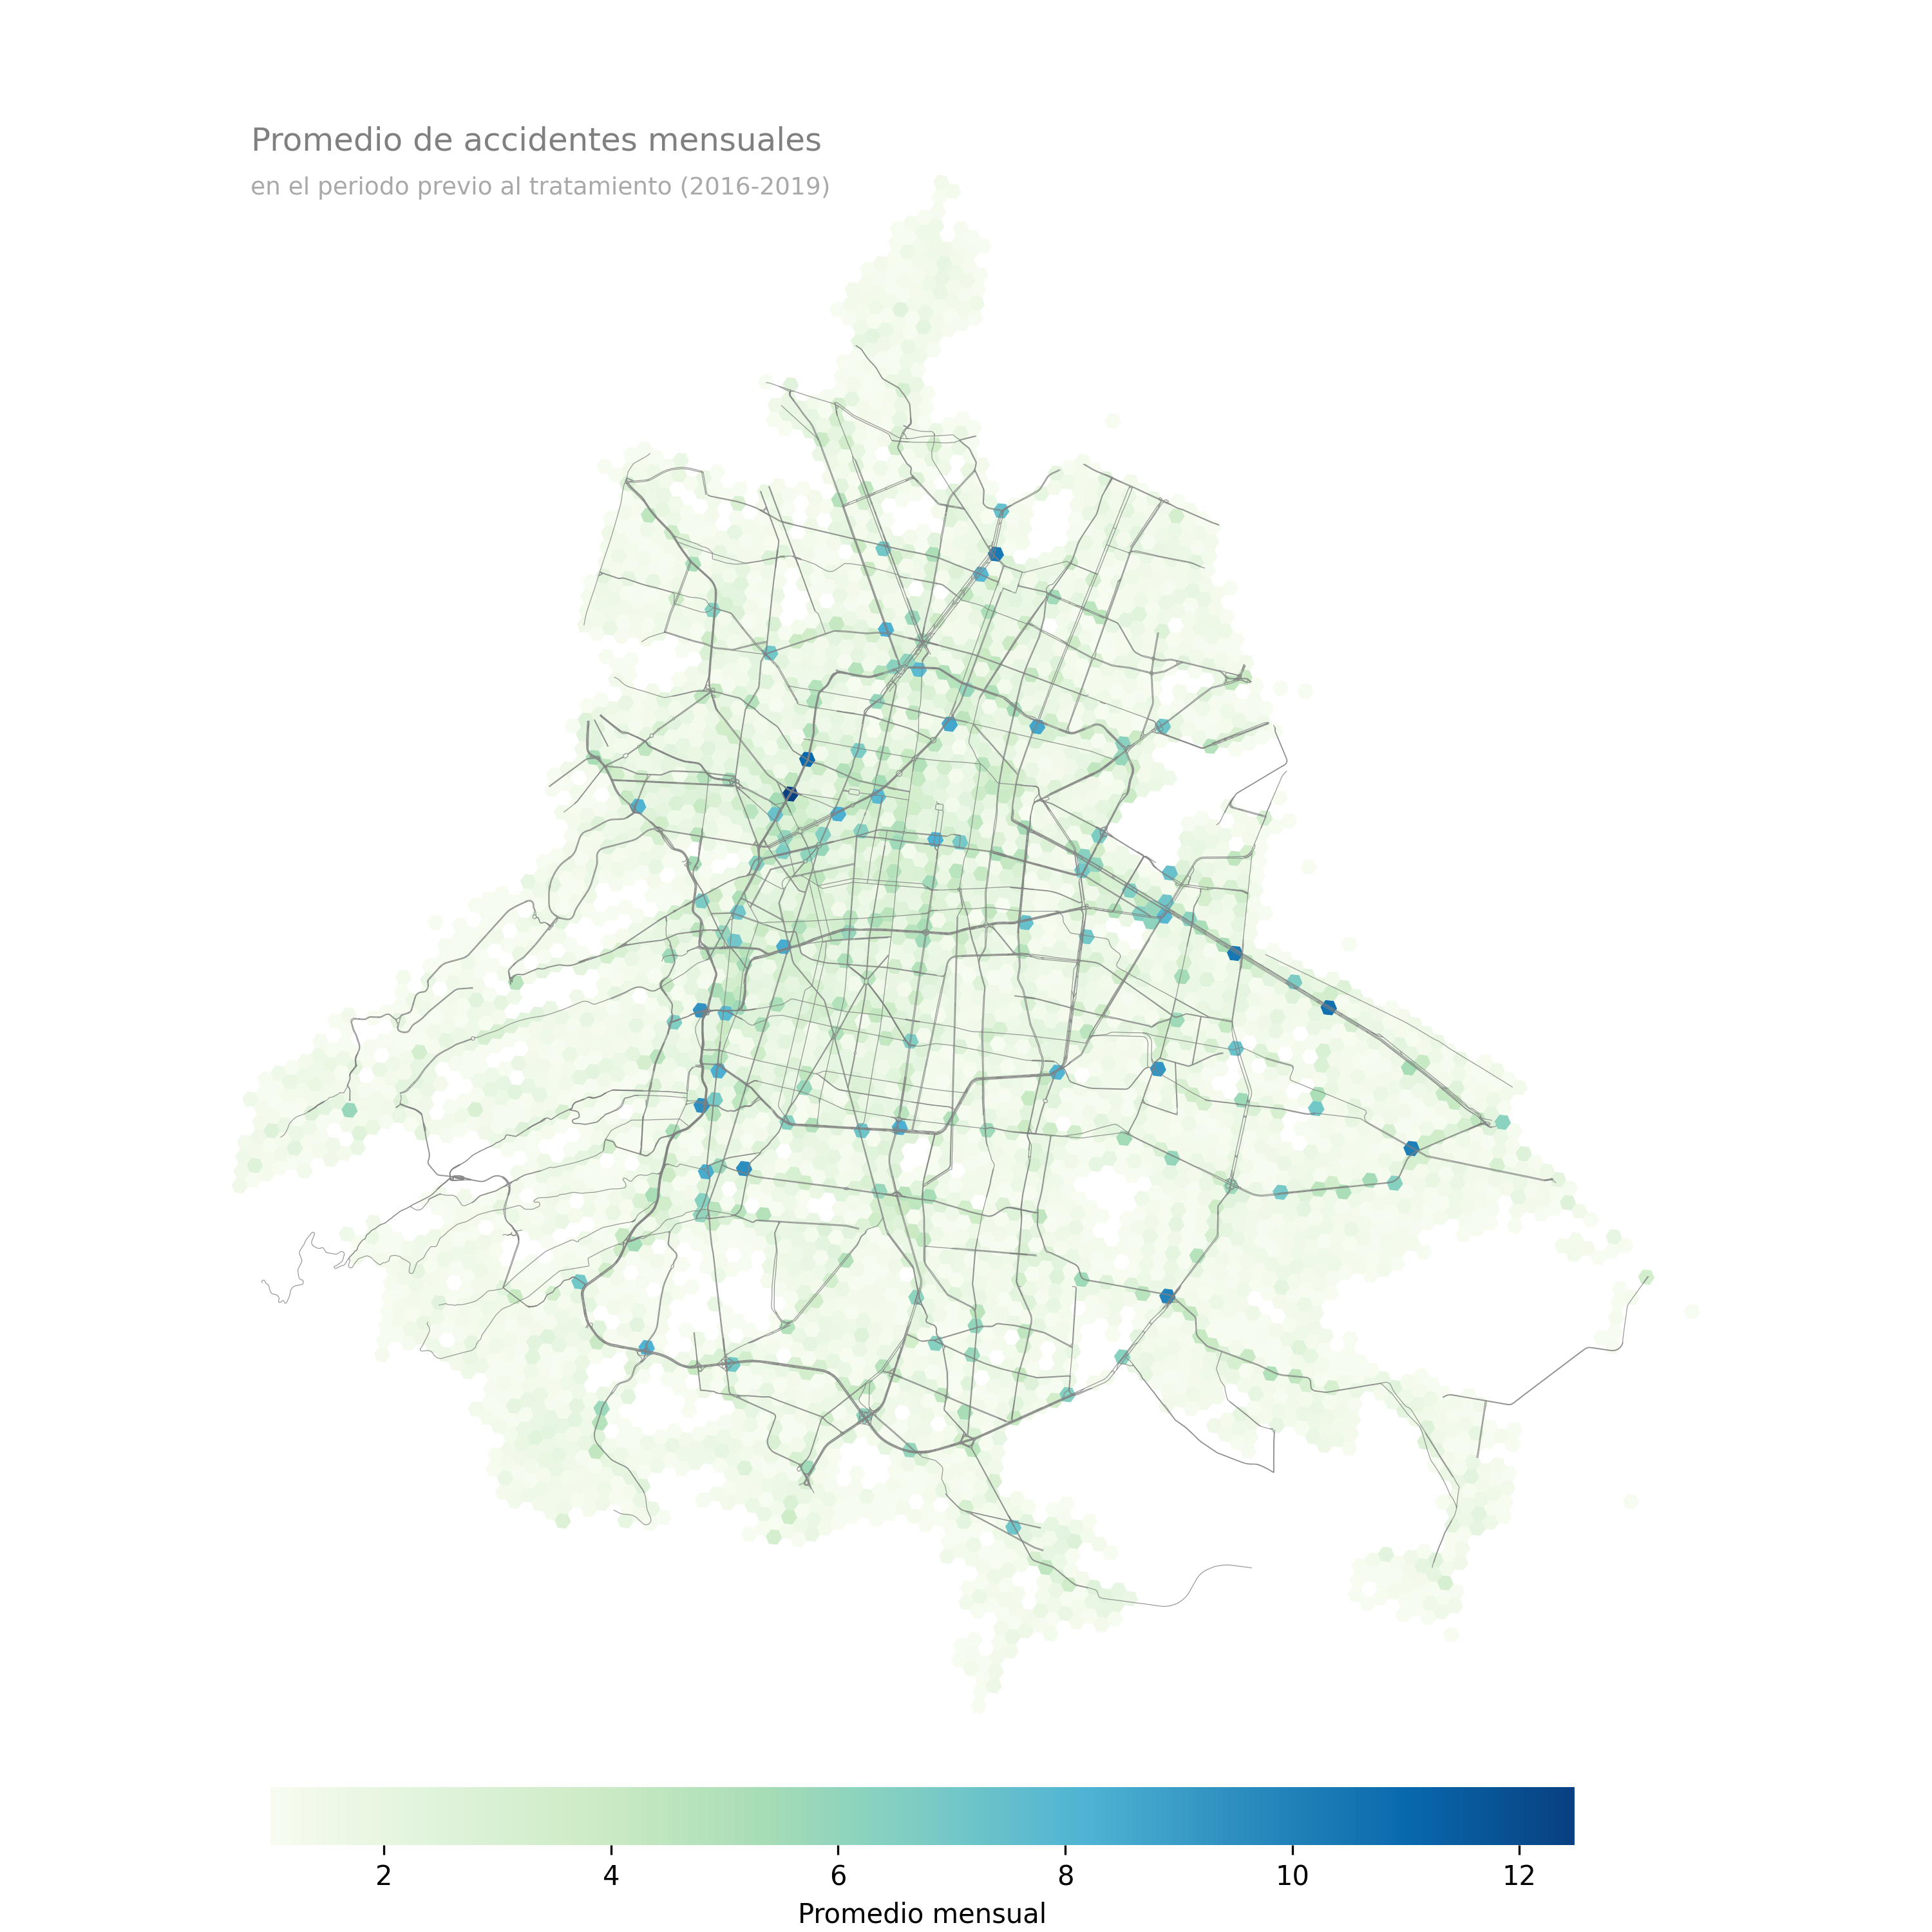
\includegraphics[width=1\linewidth]{Imagenes/promedio-accidenes-mensuales-pre-tratamiento-choroplet.png}
\end{figure}

\begin{figure}
    \centering
    \caption{Distribución de promedio de accidentes mensuales (2016-2019)}
    \label{fig:accidentes-hexagonos-dist}
    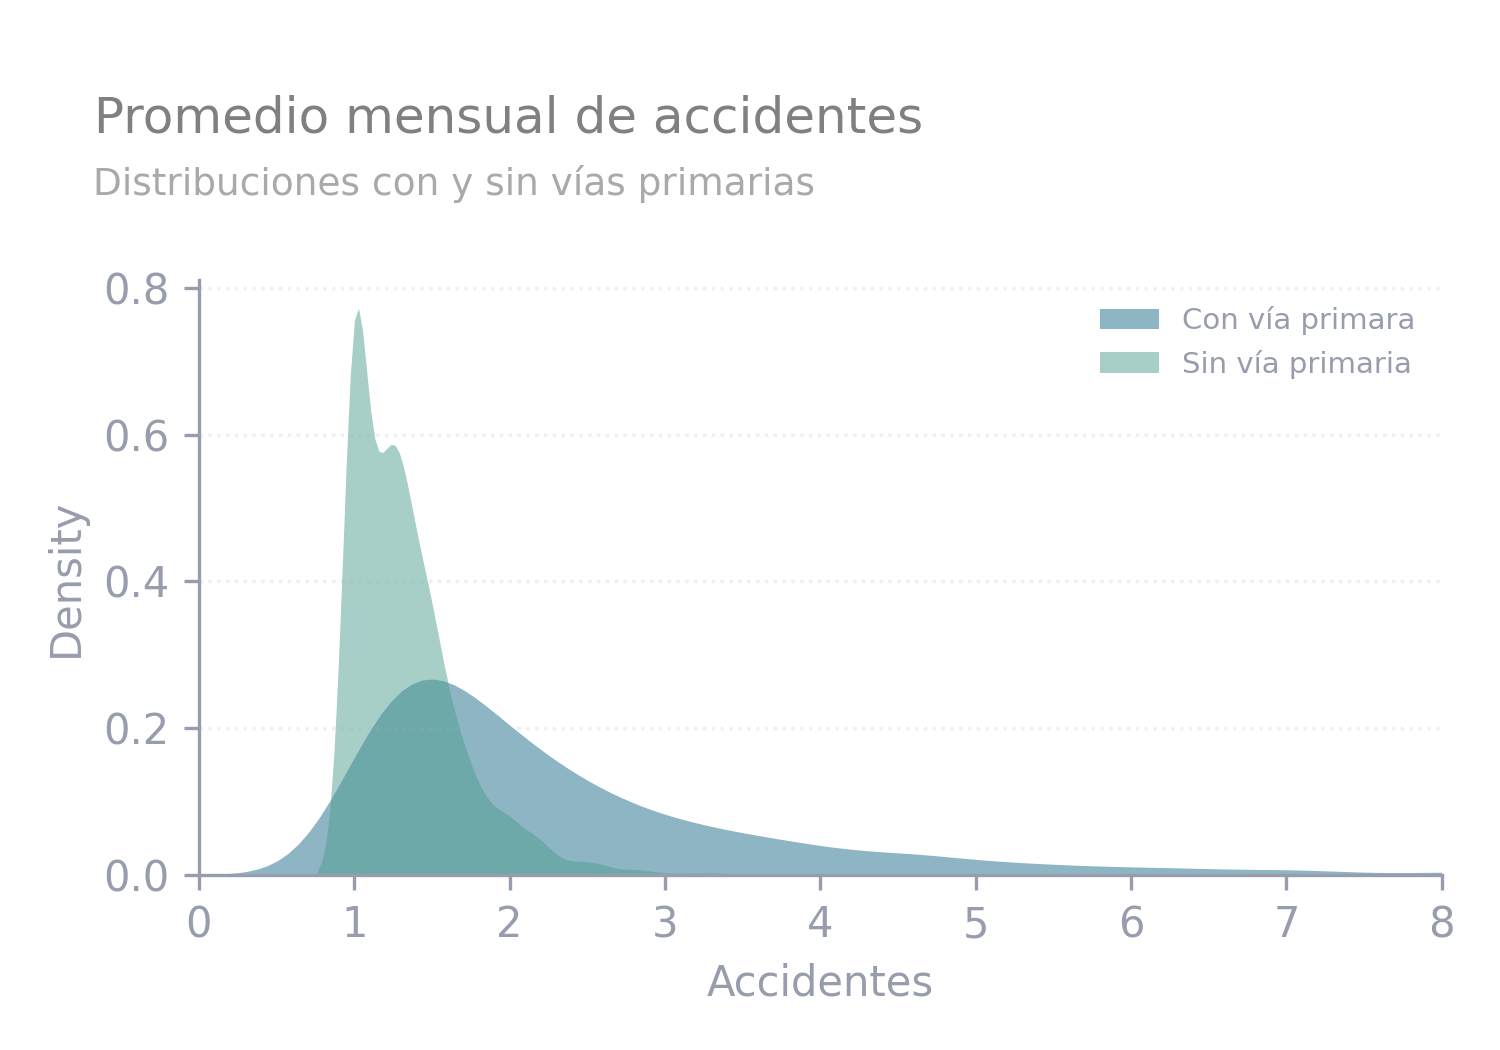
\includegraphics[width=.6\linewidth]{Imagenes/distribucion-promedio-mensual-accidentes-hexagonos.png}
\end{figure}

Por último, las zonas con vías primarias tienden a presentar un perfil de uso de suelo distinto. Para aproximar la intensidad de actividad comercial y de servicios, utilizo la API de \emph{Places Aggregate} de Google para obtener el número de establecimientos por hexágono (de la misma dimensión que el análisis de accidentes). Se diseñó una lista de categorías de lugares que ayudaran a tener una representación general de cada área \footnote{Lista de categorías utilizadas en la llamada a la API de Google Places Aggregate: \texttt{restaurant}, \texttt{cafe}, \texttt{shopping\_mall}, \texttt{supermarket}, \texttt{convenience\_store}, \texttt{grocery\_store}, \texttt{store}, \texttt{gas\_station}, \texttt{bank}, \texttt{atm}, \texttt{hospital}, \texttt{pharmacy}, \texttt{school}, \texttt{gym}, \texttt{night\_club}, \texttt{transit\_station}, \texttt{bus\_station}, \texttt{subway\_station}.}. En promedio, los hexágonos con vías primarias concentran $77.79$ establecimientos (desviación estándar $69.10$), mientras que los hexágonos sin vías primarias tienen en promedio $56.85$ establecimientos (desviación estándar $63.36$). Si bien la variabilidad es alta y la mayor concentración de negocios se observa en torno al centro de la ciudad, existe una diferencia promedio consistente entre ambos tipos de zonas (Figuras~\ref{fig:establecimientos-dist} y~\ref{fig:establecimientos-mapa}).\\

\begin{figure}
    \centering
    \caption{Distribución del número de establecimientos por hexágono}
    \label{fig:establecimientos-dist}
    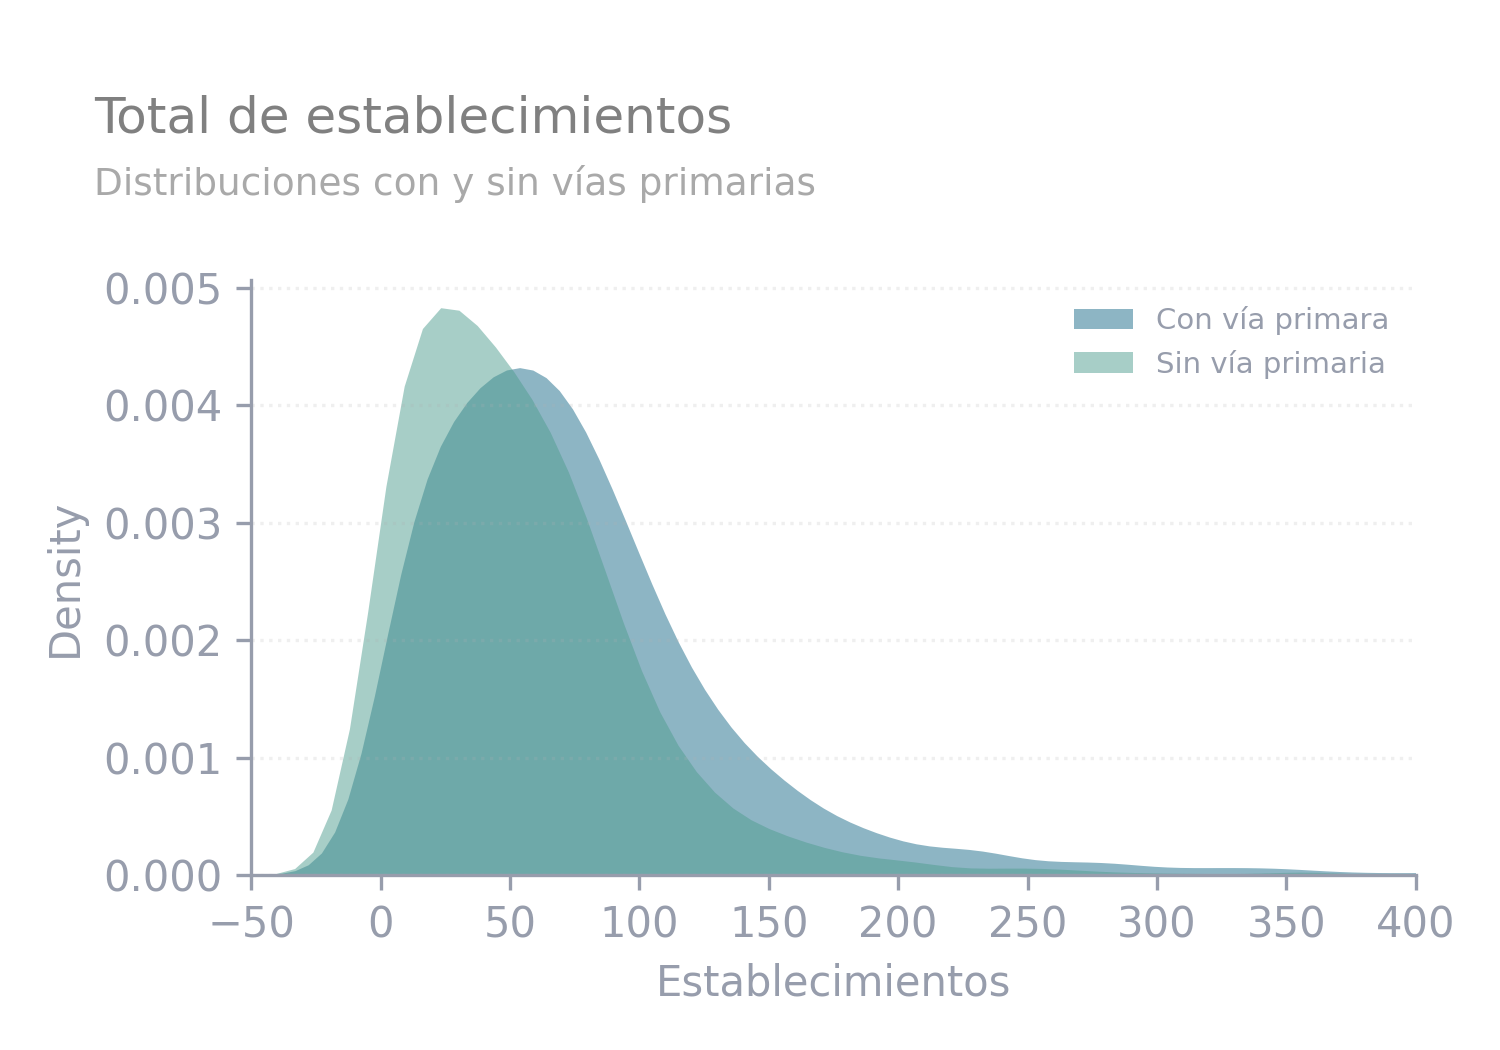
\includegraphics[width=.6\linewidth]{Imagenes/distribucion-establecimientos-cdmx-hexagonos.png}
\end{figure}

\begin{figure}
    \centering
    \caption{Establecimientos en la CDMX}
    \label{fig:establecimientos-mapa}
    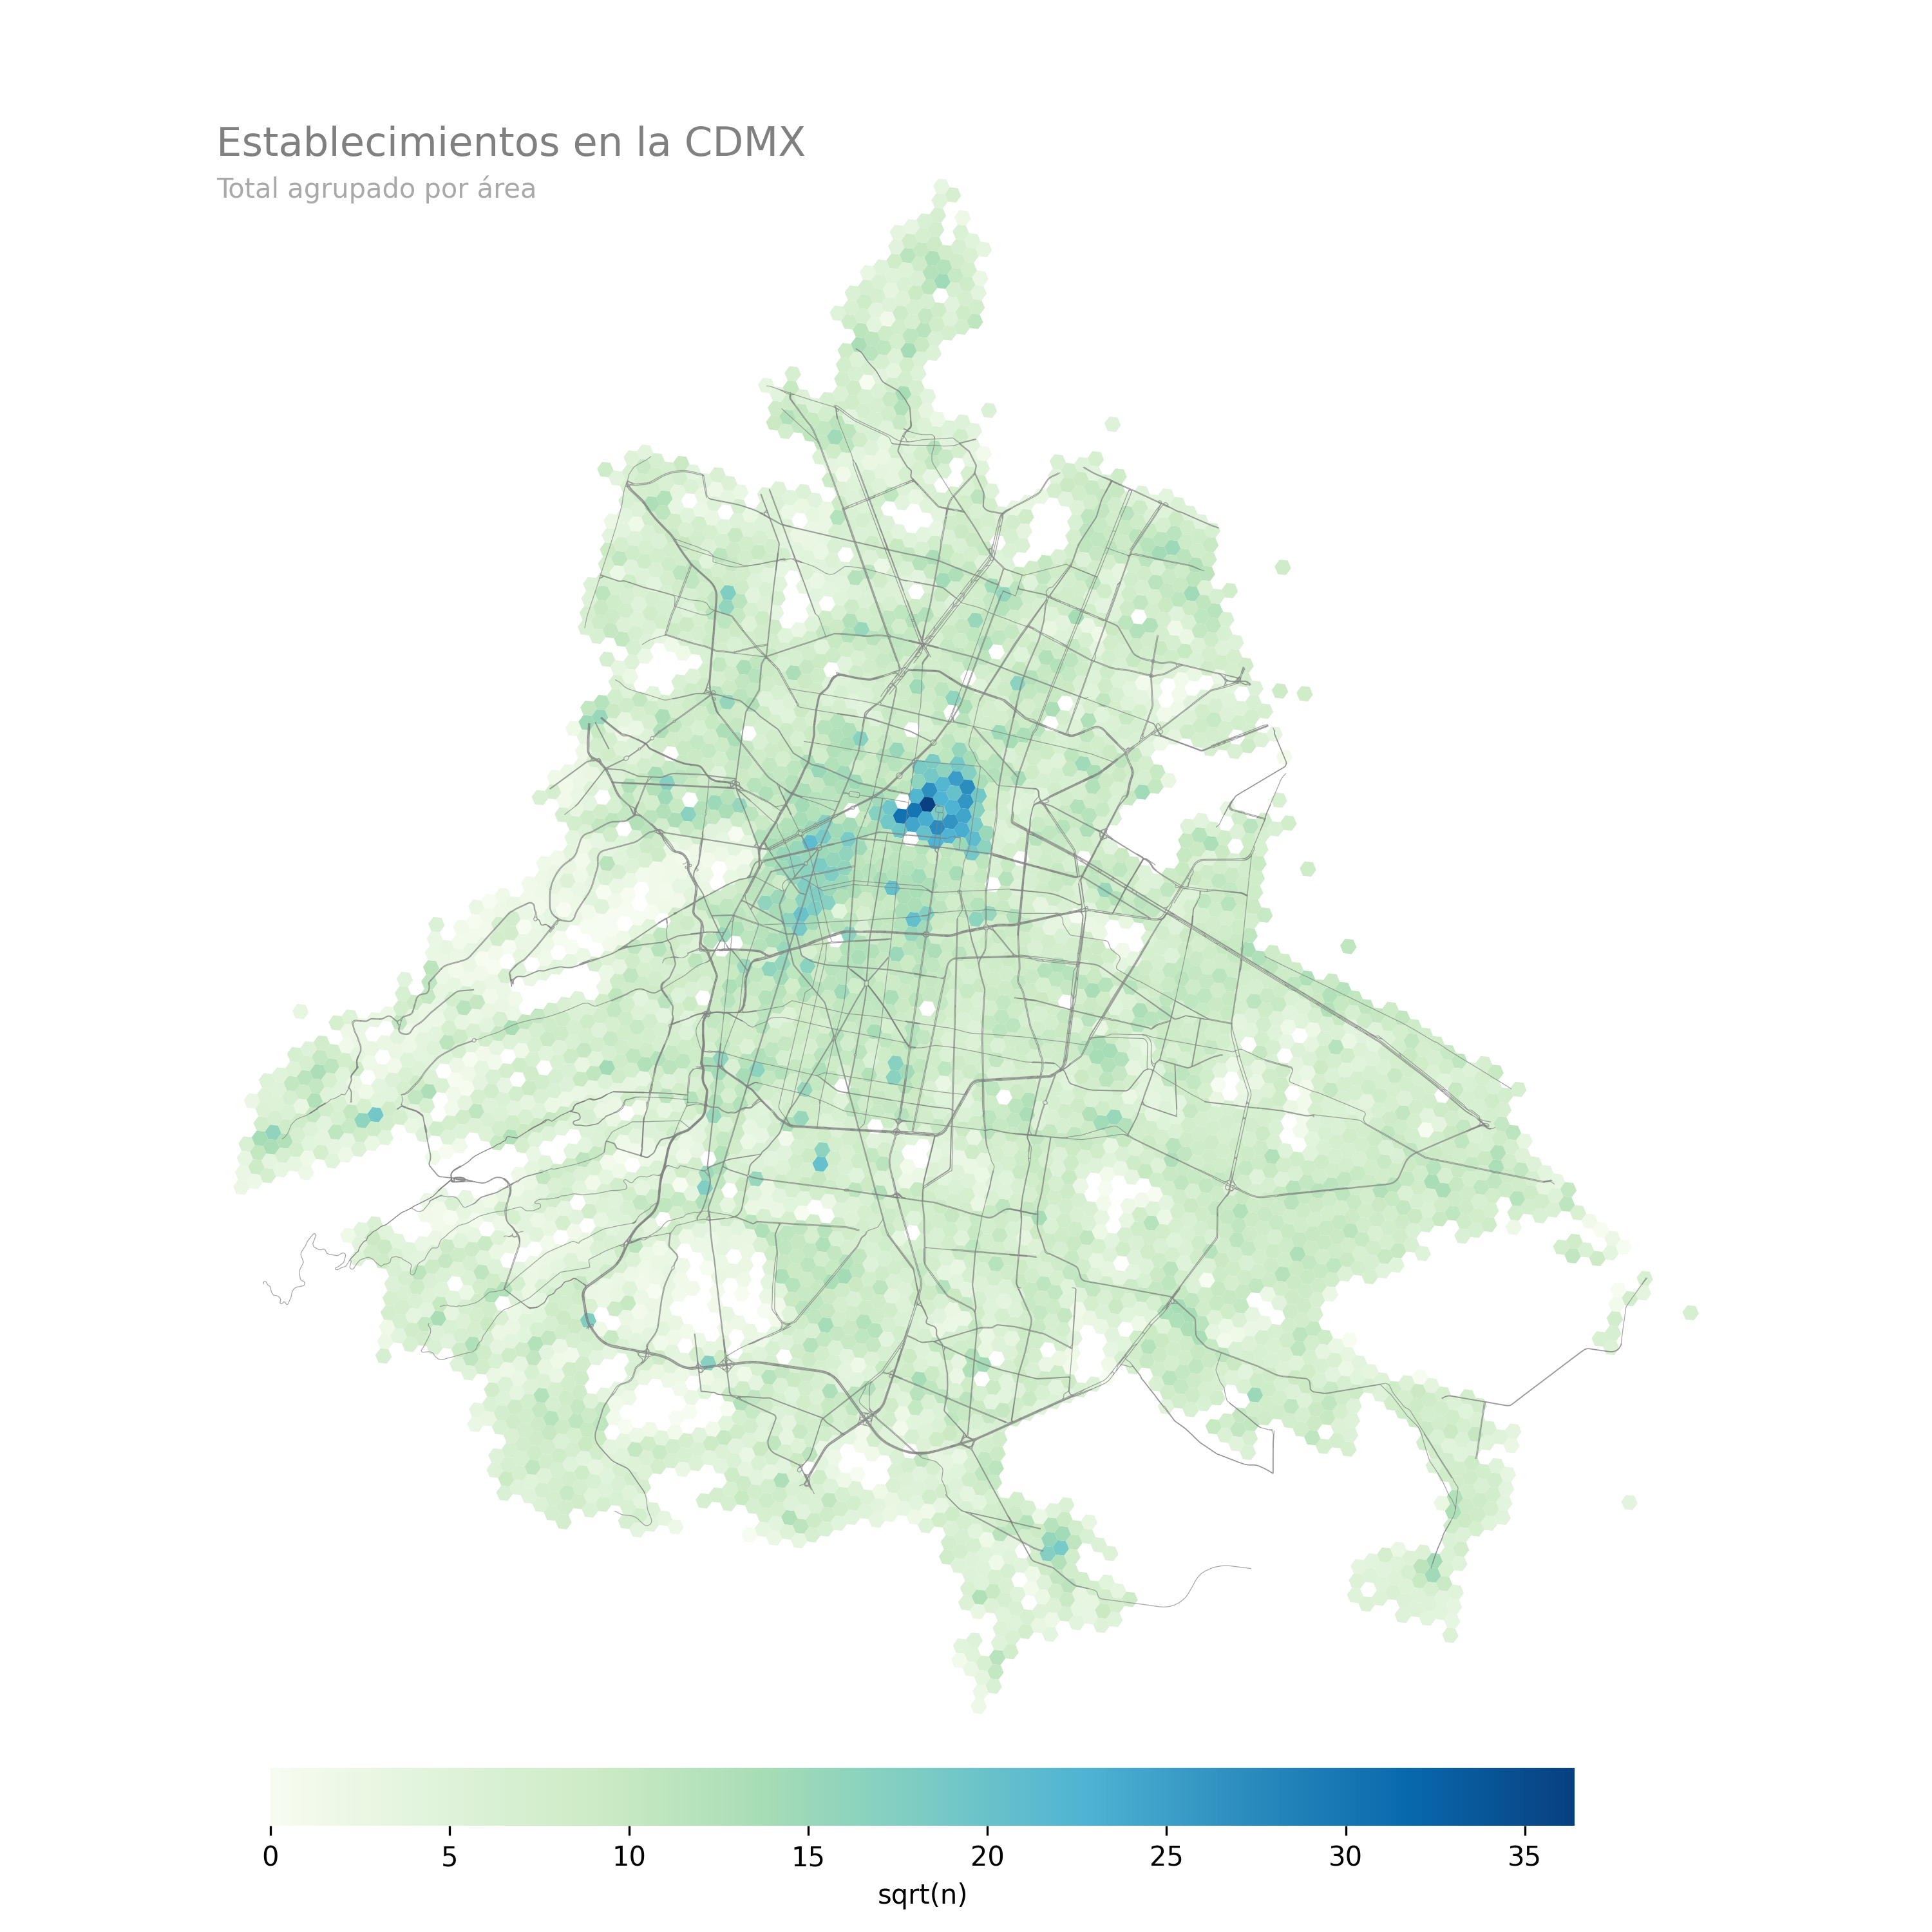
\includegraphics[width=1\linewidth]{Imagenes/establecimientos-en-la-cdmx.png}
\end{figure}
En conjunto, estas diferencias en velocidad reglamentaria, siniestros y nivel de actividad económica muestran que las zonas con y sin vías primarias corresponden a entornos viales y urbanos cualitativamente distintos. Una comparación directa entre ellas introduciría sesgos difíciles de manejar, incluso tras ajustar por covariables observables. Por este motivo, acoto el universo de análisis a áreas centradas sobre vías primarias y de acceso controlado. Con base en este universo más homogéneo, más adelante implemento un procedimiento de emparejamiento por \textit{propensity score}, que selecciona de entre los candidatos los controles más parecidos a cada unidad tratada y define la muestra final del análisis.

\section{Estrategia de identificación}

\subsection{Efecto de interés}
\noindent El objetivo de esta tesis es estimar el efecto causal de las cámaras de velocidad sobre la seguridad vial en su entorno inmediato. En particular, me interesa cuantificar cómo cambia el número mensual de incidentes viales en las áreas donde se ubican los radares, en comparación con lo que hubiera ocurrido en ausencia de cámaras. El efecto se estima por separado para el total de incidentes y para cada nivel de severidad, y para cada uno de los cinco radios.\\

En términos de inferencia causal, este efecto se interpreta como un \emph{average treatment effect on the treated} (ATT): el efecto promedio de contar con una cámara sobre las áreas efectivamente tratadas, tomando como contrafactual áreas de control emparejadas con características observables similares. Conviene precisar desde ahora sobre qué áreas tratadas se define este promedio. Como se explica más adelante, el análisis solo incluye a las áreas tratadas que encuentran un control comparable en los cinco radios, de modo que el ATT corresponde a ese subconjunto y no necesariamente a todas las cámaras del programa. En el capítulo 3 se describe cuántas áreas quedan fuera y en qué se distinguen de las demás.\\

\subsection{Alternativas de estimación}
\noindent Existen, en principio, varias formas alternativas de aproximarse a este problema. Una opción natural sería un ejercicio tipo \emph{before--after} en las áreas donde se instalaron las cámaras, comparando directamente el nivel de siniestros antes y después de abril de 2019. Sin embargo, esta aproximación es especialmente problemática en este contexto por dos razones. Primero, el periodo de estudio incluye el choque exógeno de la pandemia de COVID-19, que alteró de manera drástica los patrones de movilidad y, por tanto, la siniestralidad vial. Un simple \emph{before--after} confundiría los efectos de la pandemia con los del programa de fotocívicas. Segundo, incluso en ausencia de la pandemia, cualquier cambio en tendencias generales de accidentes en la ciudad podría ser erróneamente atribuido a las cámaras si no se cuenta con un grupo de comparación adecuado.\\

Otra alternativa sería estimar un modelo de diferencia en diferencias utilizando como controles todas las áreas elegibles que no recibieron cámaras. Sin embargo, como se discutió en la sección anterior, la asignación del programa no fue aleatoria: por diseño, las cámaras se instalaron en zonas con mayor riesgo vial. Usar de manera indiscriminada todas las demás áreas como contrafactual llevaría a comparar zonas sistemáticamente más peligrosas con otras estructuralmente distintas, y no hay razón para suponer que ambos grupos hubieran seguido trayectorias similares en ausencia del programa; es decir, el supuesto de tendencias paralelas resulta poco creíble.\\

Una tercera opción sería usar únicamente \emph{propensity score matching} (PSM): emparejar cada área tratada con un área de control parecida y comparar sus incidentes después del programa. El problema es que esa comparación mira un solo momento. Las cámaras empezaron a operar en una fecha concreta y se cuenta con información de las mismas áreas antes y después de esa fecha; perderíamos información muy valiosa si no consideráramos la naturaleza temporal de la intervención, por ejemplo, cualquier diferencia entre tratadas y controles que ya existiera antes del programa y que el emparejamiento no haya eliminado. Por ello, resulta más natural combinar el emparejamiento con un modelo de diferencia en diferencias.\\

En el capítulo 4 evalúo estas posibilidades con los mismos datos, para mostrar cuánto cambia la conclusión conforme se corrigen sus problemas, hasta llegar a la especificación principal.\\

\subsection{Emparejamiento}
\noindent La estrategia de esta tesis combina ambas herramientas: primero, utilizo el \emph{propensity score} para construir pares de áreas tratadas y de control que sean lo más comparables posible en términos de covariables observables; después, estimo sobre esta muestra emparejada un modelo de diferencia en diferencias con efectos fijos. De esta manera, el emparejamiento actúa como un paso previo que mejora la calidad del grupo de comparación, mientras que la estructura de panel permite aislar los cambios diferenciales en el tiempo asociados a la implementación del programa.\\

El \emph{propensity score} es la probabilidad de que un área cuente con una cámara de velocidad, condicional en sus covariables observables. Lo estimo con un modelo logístico cuyos regresores son características del área medidas antes del programa: su infraestructura vial, su siniestralidad en los tres años previos, incluida la tendencia de los incidentes, y la afluencia del Metro. El \emph{propensity score} resume así, en una sola dimensión, la información de las covariables relevantes para la asignación de las cámaras.\\

A partir del \emph{propensity score}, cada área tratada se empareja con el área de control más parecida, sin reemplazo, de modo que cada control se utiliza a lo más una vez. Esto garantiza que cada control represente un contrafactual similar a su área tratada, en lugar de reutilizar en exceso un pequeño conjunto de controles ``muy buenos'', lo que concentraría la inferencia en pocas zonas de la ciudad. Las áreas tratadas que no encuentran ningún control suficientemente parecido se excluyen, porque para ellas no existe una comparación defendible; este es el supuesto de soporte común. Como el emparejamiento se repite en cada radio, solo se conservan las áreas tratadas que encuentran pareja en los cinco, de modo que todos los radios estiman el efecto sobre las mismas unidades. El modelo logístico, el criterio de similitud y la evaluación del balance se detallan en el capítulo 3.\\

\subsection{Especificación}
\noindent Sobre la muestra emparejada estimo tres especificaciones de manera progresiva. La primera no incluye efectos fijos:
\begin{equation}
    Y_{it} = \alpha + \delta \, T_i + \lambda \, \text{Post}_t + \beta \, (T_i \times \text{Post}_t) + \varepsilon_{it}
    \label{eq:did1}
\end{equation}
donde $Y_{it}$ es el número de incidentes en el área $i$ durante el periodo $t$; $T_i$ indica si el área es tratada, y $\text{Post}_t$ indica si el periodo es posterior al 22 de abril de 2019. En ella, $\alpha$ es el promedio de los controles antes del programa, $\delta$ la diferencia entre tratadas y controles antes del programa, $\lambda$ el cambio de los controles después del programa y $\beta$, el coeficiente de interés, el cambio adicional que registraron las tratadas por encima del de sus controles.\\

La segunda introduce efectos fijos, tanto por área como por periodo, y se quitan los indicadores de tratamiento y de periodo posterior:
\begin{equation}
    Y_{it} = \alpha_i + \lambda_t + \beta \, (T_i \times \text{Post}_t) + \varepsilon_{it}
    \label{eq:did2}
\end{equation}
donde $\alpha_i$ son efectos fijos por área, que capturan las características de cada área que no cambian en el tiempo, y $\lambda_t$ son efectos fijos por periodo, que capturan lo que le ocurre a todas las áreas en un mismo periodo. Como el panel está balanceado y todas las cámaras entraron en vigor el mismo día, $\beta$ es idéntico en las ecuaciones~\eqref{eq:did1} y~\eqref{eq:did2}.\\

La tercera, que es la especificación principal, agrega covariables interactuadas con el periodo posterior:
\begin{equation}
    Y_{it} = \alpha_i + \lambda_t + \beta \, (T_i \times \text{Post}_t) + \sum_{k=1}^{8} \gamma_k \, (X_{ik} \times \text{Post}_t) + \varepsilon_{it}
    \label{eq:did}
\end{equation}
donde $X_{ik}$ son ocho características de cada área. En las tres especificaciones el modelo es lineal y se estima por mínimos cuadrados ordinarios, de modo que $\beta$ se interpreta directamente en incidentes por mes; para facilitar su lectura, se reporta también como porcentaje del promedio mensual de incidentes del grupo de control antes del programa.\\

Las covariables se agregan porque el emparejamiento no deja un balance perfecto: después de emparejar persisten diferencias pequeñas en algunas covariables, y si esas características influyen en cómo evolucionan los incidentes después de 2019, podrían confundirse con el efecto de las cámaras. Estas covariables describen cada área antes del programa: las de infraestructura vial salen de la red vial, y la de afluencia del Metro es el promedio de los tres años previos. Cada una tiene un solo valor por área, que no se actualiza después de abril de 2019. Esto es deliberado: si las cámaras modificaron, por ejemplo, el tránsito o la afluencia del Metro a su alrededor, usar los valores posteriores al programa como control absorbería parte del efecto que se busca medir. Al ser fijas en el tiempo, por sí solas las absorben los efectos fijos de área; lo que aporta información es su interacción con $\text{Post}_t$, que permite que áreas con distinta infraestructura vial o distinta afluencia del Metro tengan cambios distintos después del programa sin atribuírselos a la cámara.\\

Por eso entran las siete covariables de infraestructura vial y la de afluencia del Metro, pero no las de siniestralidad previa: interactuar el nivel previo de incidentes con el periodo posterior equivaldría a suponer que ese nivel determina la evolución posterior, que es justamente lo que el supuesto de tendencias paralelas establece que no ocurre. Las covariables de siniestralidad se balancean en el emparejamiento, pero no entran al modelo.\\

Los efectos fijos por periodo no son un control de la pandemia. Capturan lo que le ocurre a todas las áreas en un mismo periodo, de modo que la parte del choque que fue común a tratadas y controles queda fuera de $\beta$, como se discutió en la sección~\ref{sec:ventana}. La parte que pudo afectar de forma distinta a ambos grupos no la quita ningún efecto fijo; se evalúa con el efecto por año que se describe más adelante.\\

\subsection{Inferencia}
\noindent Los errores estándar se agrupan por componente traslapada. Algunas áreas tratadas se traslapan parcialmente sin llegar a fusionarse, y registran algunos de los mismos incidentes, por lo que no son observaciones independientes. Cada grupo de áreas tratadas conectadas por algún traslape forma un \emph{cluster}; los controles, que no se traslapan con ninguna otra área, forman cada uno el suyo.\\

Estos errores estándar, sin embargo, tratan los pares emparejados como si fueran fijos, cuando en realidad se construyeron con los mismos datos: con otra muestra, el \emph{propensity score} sería distinto y el emparejamiento elegiría otros controles. Para incorporar esa incertidumbre, calculo los intervalos de confianza con un \emph{bootstrap} que repite el proceso completo. En cada una de 2,000 repeticiones se remuestrean, con reemplazo, las áreas tratadas y el conjunto de controles candidatos, de modo que las áreas de un mismo \emph{cluster} entran o salen juntas; sobre esa muestra se vuelve a estimar el modelo logístico, se rehace el emparejamiento con las mismas reglas y se estima de nuevo el modelo de diferencia en diferencias. El intervalo de confianza al 95\% se construye con los percentiles 2.5 y 97.5 de los coeficientes obtenidos. Las limitaciones de este procedimiento se discuten en las conclusiones.\\

\subsection{Evaluación de los supuestos}
\noindent El supuesto de tendencias paralelas no puede probarse directamente, porque se refiere a lo que hubiera ocurrido sin el programa. Lo que sí puede revisarse es si tratadas y controles ya se separaban antes de 2019. Para ello hago un \emph{event study}: la misma especificación~\eqref{eq:did}, pero con un coeficiente de tratamiento para cada año de la ventana, anterior o posterior al programa, y con el año inmediatamente anterior a las fotocívicas como referencia. Las covariables también se interactúan con cada año. Si las tendencias eran paralelas, los coeficientes de los años previos deberían ser cercanos a cero; además de revisarlos uno por uno, se prueba conjuntamente que todos sean cero.\\

Como ya se adelantaba, verifico también que la pandemia no esté cargando los resultados. Para esto, estimo una variante en la que el indicador $\text{Post}_t$ se separa en tres indicadores anuales, cada uno del 22 de abril al 21 de abril del año siguiente: el primero cierra con el primer mes del confinamiento, el segundo corresponde al año de la pandemia y el tercero va de 2021 a 2022. Si el efecto estimado se debiera a un choque de la pandemia que afectó de forma distinta a tratadas y controles, el coeficiente del segundo año debería apartarse de los demás. Los resultados de ambas pruebas se presentan en el capítulo 4.\\


\chapter{Datos y balance}
\label{chap:datos}

\noindent Este capítulo describe los datos con los que se construye el análisis y la muestra sobre la que se estima el efecto de las cámaras. La primera sección presenta las fuentes, organizadas según el papel que cumple cada variable: el tratamiento, la siniestralidad, la infraestructura vial y el Metro. Para cada fuente se describe qué contiene, cómo se limpió y qué variables se construyen a partir de cada una. La segunda sección especifica cómo se construyen las unidades tratadas y los controles, y cuántas unidades quedan en cada paso. La tercera describe el modelo del \emph{propensity score} y las reglas del emparejamiento, y evalúa el soporte común y el balance de la muestra final. La última contiene las limitaciones de los datos.

\section{Fuentes y variables}

\subsection{Tratamiento}

\noindent La ubicación de las cámaras proviene del conjunto de datos \emph{Fotoc\'ivicas (Ubicación)} de la Secretaría de Seguridad Ciudadana (SSC, 2023), publicado en el portal de datos abiertos de la Ciudad de México. Para cada una de las 113 cámaras del programa reporta la vialidad, el cruce en el que se encuentra, el sentido de circulación que vigila y sus coordenadas. A diferencia del esquema de fotomultas, la ubicación de las cámaras de fotocívicas es pública, lo que permite identificar con precisión las zonas tratadas.\\

Las 113 cámaras se conservan sin limpieza. Tres pares de cámaras comparten exactamente la misma coordenada.\footnote{Son los registros 7 y 8, ambos descritos en el cruce de Insurgentes y Eje 1 Norte, en Buenavista; 5 y 25, descritos en Universidad y Miguel Ángel de Quevedo y en Eje 5 Sur y Anillo Periférico Oriente, y 52 y 53, descritos sobre la Autopista Urbana Norte a la altura de Constituyentes y de Ejército Nacional. En los dos últimos pares, la coordenada coincide con el cruce de la primera cámara: está a 40 metros de la estación Miguel Ángel de Quevedo del Metro y a 200 metros del cruce de Constituyentes con el Periférico. Los cruces descritos para las cámaras 25 y 53 están a 13 y 4 kilómetros de la coordenada, respectivamente.} En el primer par se trata de dos cámaras en el mismo cruce, una para cada sentido. En los otros dos, el cruce que describe la fuente para una de las cámaras está a varios kilómetros de la coordenada registrada, es decir, la fuente le asignó la coordenada de la otra cámara. Como no hay forma de conocer su ubicación exacta, cada par se trata como cualquier otro par de cámaras cercanas: se agrupan en una sola unidad tratada (sección~\ref{sec:unidades}).\\

A partir de estas ubicaciones se define el indicador de tratamiento $T_i$, que vale uno si el área $i$ contiene al menos una cámara y cero si es un control.

\subsection{Siniestralidad}

\noindent Los incidentes viales provienen del conjunto de datos \emph{Incidentes viales reportados por C5} del Centro de Comando, Control, Cómputo, Comunicaciones y Contacto Ciudadano de la Ciudad de México (C5, 2024). Cada registro corresponde a un folio de atención, con su fecha, hora, coordenadas, tipo de incidente y la clasificación con la que se cerró. Se prefiere esta fuente frente a los registros de la SSC por dos razones. La primera es su cobertura temporal: los datos de la SSC solo tienen coordenadas geográficas a partir de junio de 2018, lo que impide construir tres años previos al programa, mientras que el C5 reporta incidentes desde diciembre de 2013. La segunda es su alcance: la base de la SSC se limita a incidentes con lesionados o fallecidos, mientras que el C5 integra llamadas al 911, botones de auxilio y videovigilancia, e incluye incidentes menores. Excluirlos impediría detectar un efecto del programa sobre la frecuencia de los incidentes, y no solo sobre su gravedad.\\

Los datos contienen 2,115,080 folios entre el 31 de diciembre de 2013 y el 29 de febrero de 2024. Para la limpieza se hizo lo siguiente:

\begin{enumerate}
    \item Se conservan los folios con código de cierre A (afirmativo), es decir, aquellos en los que una unidad de emergencia llegó al lugar y confirmó el incidente. Quedan 866,230.
    \item Se recorta la ventana del análisis, del 22 de abril de 2016 al 21 de abril de 2022. Quedan 433,235.
    \item Se conservan los incidentes tipificados como \emph{Accidente}, \emph{Cadáver} o \emph{Lesionado}, sin la clasificación de falsa alarma, para descartar llamadas que no corresponden a hechos de tránsito. Quedan 432,707.
    \item Se eliminan cuatro folios repetidos y cinco registros con coordenadas en cero. Quedan 432,698.
\end{enumerate}

Los incidentes se clasifican en tres niveles mutuamente excluyentes según su gravedad: fatales (FCS), si se registró un cadáver en el lugar, con 1,957 incidentes; con lesionados (PIC), si la clasificación de la alarma fue de urgencias médicas, con 191,676, y menores (MIN), sin lesionados ni fallecidos, con 239,065.\\

\textbf{Variable de resultado}. La variable de resultado $Y_{it}$ es el número de incidentes en el área $i$ durante el periodo $t$, tanto el total como para cada nivel de severidad. Los periodos van del día 22 de un mes al 21 del siguiente, de modo que el corte del 22 de abril de 2019 coincide con el inicio de un periodo, y la ventana tiene 36 periodos antes del programa y 36 después. Un incidente que cae en el área compartida por dos o más áreas tratadas se reparte en partes iguales entre ellas, como se detalla en la sección~\ref{sec:unidades}.\\

\textbf{Covariables de siniestralidad}. La misma fuente da lugar a cuatro covariables, que describen la siniestralidad de cada área en los tres años previos al programa. Se consideran los años hacia atrás a partir del 22 de abril de 2019: el año $-1$ va del 22 de abril de 2018 al 21 de abril de 2019, y así sucesivamente.

\begin{itemize}
    \item \textbf{Nivel de incidentes} (\texttt{nivel\_incidentes}): promedio mensual de incidentes de todos los niveles en los tres años previos.
    \item \textbf{Proporción con lesionados} (\texttt{pct\_lesionados}): fracción de esos incidentes que tuvo consecuencias personales; incluye tanto PIC como FCS.
    \item \textbf{Tendencia} (\texttt{tendencia}): promedio mensual de incidentes del año $-1$ menos el del año $-3$. Un valor positivo indica que los incidentes del área venían en aumento antes del programa, y uno negativo, que venían a la baja.
    \item \textbf{Algún incidente fatal} (\texttt{hubo\_fcs}): indicador de que el área registró al menos un incidente fatal en los tres años previos. Se usa un indicador y no un conteo porque los incidentes fatales son poco frecuentes: en un año dado, entre el 58\% y el 84\% de las áreas no registra ninguno.
\end{itemize}

Con estas covariables se representan los factores que consideró la Secretaría de Movilidad al reubicar las cámaras, cuando se priorizaron los lugares donde los incidentes eran más frecuentes y más graves (SEMOVI, 2019). La tendencia, además, permite que el emparejamiento compare áreas cuya siniestralidad venía evolucionando de forma parecida antes del programa, lo que sirve directamente al supuesto de tendencias paralelas del modelo de diferencias en diferencias.

\subsection{Infraestructura vial}

\noindent Las características de la red vial provienen del conjunto de datos \emph{Vialidades primarias de la Ciudad de México} de la Secretaría de Movilidad (SEMOVI, 2023). Contiene los tramos de las vías primarias y de acceso controlado de la ciudad, con el número de carriles, el sentido de circulación, el tipo de vía y el nivel en el que corre cada tramo: a nivel de calle, elevado o subterráneo. En total se identifican 149 vialidades: 135 con tramos de vía primaria y 21 con tramos de acceso controlado, ya que siete tienen tramos de ambos tipos. La misma red sirve para sortear los centros de los controles (sección~\ref{sec:controles}).\\

A partir de ella se construyen siete covariables, ponderadas por los metros de vía que caen dentro de cada área:

\begin{itemize}
    \item \textbf{Longitud vial} (\texttt{road\_length\_m}): metros de vía dentro del área.
    \item \textbf{Número de vialidades} (\texttt{n\_vialidades}): vialidades distintas que cruzan el área.
    \item \textbf{Carriles ponderados} (\texttt{carriles\_ponderados}): número promedio de carriles, ponderado por los metros de cada tramo.
    \item \textbf{Acceso controlado} (\texttt{pct\_acceso\_controlado}): fracción de los metros de vía que corresponde a vías de acceso controlado.
    \item \textbf{Doble sentido} (\texttt{pct\_doble\_sentido}): fracción de los metros de vía en tramos de doble sentido.
    \item \textbf{Desnivel} (\texttt{pct\_desnivel}): fracción de los metros de vía en tramos elevados o bajo el suelo.
    \item \textbf{Número de niveles} (\texttt{n\_niveles}): niveles distintos que se encuentran dentro del área.
\end{itemize}

Las covariables se ponderan por longitud porque así describen la composición de toda el área, y no solo la vía más grande que la cruza: un círculo atravesado por unos metros de una avenida de seis carriles no se parece a uno recorrido por ella de lado a lado. No se incluye la fracción de vía primaria porque, al contener la capa solo vías primarias y de acceso controlado, es igual a uno menos la fracción de acceso controlado. Las dos últimas covariables miden la ambigüedad vertical de cada área, que se discute en la sección~\ref{sec:limitaciones}.

\subsection{Metro}

\noindent La información del Metro combina dos fuentes de la Secretaría de Movilidad. La primera es la capa geográfica \emph{Ubicación de líneas y estaciones del Sistema de Transporte Colectivo Metro} (SEMOVI, 2026), con la ubicación de las estaciones. Tiene 195 registros para 163 estaciones, porque las estaciones de transbordo tienen un registro por línea. La segunda es la \emph{Afluencia diaria del Metro CDMX} (SEMOVI, 2025), que reporta el número de usuarios por día, línea y estación desde 2010.\\

Para poder unir ambas fuentes fue necesario corregir el nombre de dos estaciones: la afluencia usa el nombre anterior de Niños Héroes, y la capa geográfica escribe ``Mixhiuca'' en lugar de Mixiuhca. Con estas correcciones, todos los pares de línea y estación de la afluencia encuentran su ubicación.\\

De estas fuentes sale una sola covariable:

\begin{itemize}
    \item \textbf{Afluencia del Metro} (\texttt{afluencia\_nivel}): promedio mensual de usuarios de las estaciones ubicadas dentro del área, en los tres años previos al programa. Vale cero si el área no contiene ninguna estación.
\end{itemize}

La afluencia funciona como un indicador de la actividad y del tránsito de personas en la zona. Basta con un solo promedio porque la afluencia de una estación casi no cambia de un año a otro: lo que distingue a las áreas es qué estación tienen. A 300 metros, el 32\% de las áreas tratadas tiene alguna estación del Metro dentro, mientras que solo el 13\% de los controles la tiene. El cero representa una zona sin Metro, no falta de información. Se prefirió esta medida a la distancia a la estación más cercana, que obligaría a suponer que una estación influye en la zona incluso cuando queda fuera del área.

\subsection{Resumen de variables}

\noindent El cuadro~\ref{tab:variables} resume las variables del análisis. Las doce covariables se miden entre el 22 de abril de 2016 y el 21 de abril de 2019, y cada una tiene un solo valor por área, que permanece fijo tras la implementación del programa. Las doce entran al modelo del \emph{propensity score}. En la especificación principal~\eqref{eq:did}, las covariables se interactúan con el periodo posterior, excepto las de siniestralidad, que se excluyen por las razones expuestas en la sección~\ref{sec:especificacion}.

\begin{table}[htbp]
    \centering
    \caption{Variables del análisis}
    \label{tab:variables}
    \footnotesize
    \begin{tabularx}{\textwidth}{l l >{\raggedright\arraybackslash}X}
        \toprule
        Variable & Fuente & Definición \\
        \midrule
        \multicolumn{3}{l}{\textit{Tratamiento y resultado}} \\
        $T_i$ & SSC & Indicador de que el área contiene al menos una cámara \\
        $Y_{it}$ & C5 & Incidentes en el área $i$ durante el periodo $t$, en total y por nivel \\
        \midrule
        \multicolumn{3}{l}{\textit{Siniestralidad previa}} \\
        \texttt{nivel\_incidentes} & C5 & Incidentes al mes, promedio de los tres años previos \\
        \texttt{pct\_lesionados} & C5 & Fracción de incidentes con lesionados o fallecidos \\
        \texttt{tendencia} & C5 & Incidentes al mes del año $-1$ menos los del año $-3$ \\
        \texttt{hubo\_fcs} & C5 & Al menos un incidente fatal en los tres años previos \\
        \midrule
        \multicolumn{3}{l}{\textit{Infraestructura vial}} \\
        \texttt{road\_length\_m} & SEMOVI & Metros de vía dentro del área \\
        \texttt{n\_vialidades} & SEMOVI & Vialidades distintas que cruzan el área \\
        \texttt{carriles\_ponderados} & SEMOVI & Carriles promedio, ponderados por metros de vía \\
        \texttt{pct\_acceso\_controlado} & SEMOVI & Fracción de los metros en vías de acceso controlado \\
        \texttt{pct\_doble\_sentido} & SEMOVI & Fracción de los metros en vías de doble sentido \\
        \texttt{pct\_desnivel} & SEMOVI & Fracción de los metros en tramos elevados o bajo el suelo \\
        \texttt{n\_niveles} & SEMOVI & Niveles distintos dentro del área \\
        \midrule
        \multicolumn{3}{l}{\textit{Movilidad}} \\
        \texttt{afluencia\_nivel} & SEMOVI & Usuarios al mes de las estaciones del Metro dentro del área; cero si no hay estación \\
        \bottomrule
    \end{tabularx}
\end{table}

\section{Unidades de análisis y muestra}

\noindent La unidad de análisis es un área circular de radio $r$, con $r \in \{100, 150, 200, 250, 300\}$ metros, observada en cada uno de los 72 periodos de la ventana. Tanto las áreas tratadas como las de control son círculos del mismo radio, lo que hace posible compararlas entre sí. A continuación se especifica cómo se definen los centros de los círculos de ambos tipos de unidades.

\subsection{Unidades tratadas}
\label{sec:unidades}

\noindent Algunas cámaras están tan cerca entre sí que sus círculos prácticamente coinciden, y tratarlas por separado contaría dos veces la misma zona. Por ello, dos cámaras se agrupan en una sola unidad tratada cuando sus círculos de 300 metros comparten más del 60\% de su área, lo que equivale a que sus ubicaciones estén a menos de 192 metros. El centro de cada unidad es el promedio de las ubicaciones de sus cámaras. Tras la construcción, las 113 cámaras quedan en 99 unidades tratadas: 87 con una sola cámara, 10 con dos y 2 con tres.\\

El conjunto de unidades tratadas se construye una sola vez, con el radio de 300 metros, y se mantiene igual en el resto de los radios. Así, siempre se habla de los mismos centros, y lo único que cambia entre estimaciones es el radio.\\

Dos condiciones acotan el umbral del 60\%. Por un lado, con un umbral de 50\% se agruparían dos cámaras separadas por 204 metros, cuyo centro queda a 102 metros de cada una: a 100 metros, esa unidad tratada no contendría ninguna cámara. Con 60\%, la cámara más alejada del centro de su unidad está a 81 metros. Por otro lado, con un umbral de 70\% se agrupan menos cámaras y aparecen círculos traslapados desde los 100 metros, mientras que con 60\% no hay ningún traslape en ese radio.\footnote{Ningún umbral evita todos los casos límite. Las unidades 32 y 77 son dos cámaras sobre el mismo tramo del segundo piso del Periférico, con sus centros a 205 metros, y quedaron separadas por 13 metros. Con un umbral de 50\%, que sí las agrupa, el efecto estimado a 300 metros en la especificación principal cambia a lo más 0.18 errores estándar en los cuatro niveles de gravedad.}\\

\textbf{Traslape entre unidades tratadas}. Con esta regla, los círculos de unidades distintas pueden traslaparse parcialmente en los radios mayores. A 100 metros no hay ningún traslape; a 300 metros, 36 unidades comparten parte de su área con alguna otra, y en esas áreas compartidas cae el 5.5\% de los incidentes. Cada incidente en un área compartida se reparte en partes iguales entre las unidades que lo contienen: cuenta $1/2$ en cada una si cae en dos círculos, $1/3$ si cae en tres, y así sucesivamente. Con este reparto, la suma de los incidentes de todas las unidades coincide con el número real de incidentes, 44,153 a 300 metros, en lugar de los 46,730 que resultarían de contar dos veces los compartidos.\\

El reparto resuelve el conteo de los incidentes, pero implica que los incidentes de unidades traslapadas dejan de ser independientes. Por ello, las unidades tratadas conectadas por algún traslape forman una \emph{componente}, que es la que se usa para agrupar los errores estándar y para remuestrear en el \emph{bootstrap}. Es importante distinguir que una componente no es una unidad de análisis: cada unidad conserva su propio círculo y su propio emparejamiento, y las componentes cambian con el radio. La figura~\ref{fig:componentes} muestra un ejemplo: las mismas cinco unidades tratadas forman cinco componentes a 100 metros, cuatro a 200 y una sola a 300. Entre las 93 unidades de la muestra final hay 93 componentes a 100 metros, 86 a 200 y 72 a 300.

\begin{figure}[htbp]
    \centering
    \includegraphics[width=\linewidth]{Imagenes/componente-tratado-100-200-300.pdf}
    \caption{Las mismas cinco unidades tratadas en tres radios}
    \label{fig:componentes}
    \begin{minipage}{0.95\linewidth}
        \footnotesize \textit{Nota:} Cada círculo es una unidad tratada, centrada en el promedio de sus cámaras. Las líneas rojas unen las unidades cuyos círculos se traslapan; las unidades conectadas forman una componente. En gris, la red de vías primarias y de acceso controlado. La escala es la misma en los tres paneles.
    \end{minipage}
\end{figure}

\subsection{Controles}
\label{sec:controles}

\noindent La construcción de los controles se hace sobre la misma red vial, considerando tanto las vías primarias como las de acceso controlado. Se colocan 20,000 puntos al azar, con probabilidad proporcional a la longitud de cada tramo, de modo que cada metro de vía tiene la misma probabilidad de recibir un punto. Se eligió esta construcción, frente a usar los cruces de la red o una malla, porque es la que menos decisiones arbitrarias requiere: no hay que definir qué cuenta como un cruce ni dónde empieza la malla, y cubre por igual los tramos y los cruces.\\

Una vez sorteados los puntos, se eliminan los que quedan a menos de 600 metros del centro de alguna unidad tratada, es decir, a menos de dos veces el radio más grande. Con esto, ningún control comparte área con una unidad tratada en ninguno de los cinco radios. Quedan 14,656 posibles controles, alrededor de 148 por cada unidad tratada, y este conjunto también se mantiene fijo para todos los radios.\\

Inicialmente se permite que los candidatos se traslapen entre sí: cada candidato representa el contrafactual de su propia zona, y exigir que no se traslaparan reduciría el conjunto a unos cientos de puntos y empeoraría el emparejamiento. Por la misma razón, los incidentes de los candidatos cuentan completos y no se reparten. La restricción se impone sobre los controles seleccionados: en el emparejamiento, ningún control puede quedar a menos de dos radios de otro control ya elegido, de modo que los controles de la muestra final no se traslapan entre sí y cada uno forma su propia componente.

\subsection{Muestra final}

\noindent Dado que las covariables se calculan dentro del círculo, el emparejamiento se hace por separado en cada radio. En cada radio, algunas unidades tratadas no encuentran un control suficientemente parecido (sección~\ref{sec:emparejamiento}): tres a 100 metros, una a 150, ninguna a 200, dos a 250 y una a 300. Para que las estimaciones de los cinco radios describan exactamente las mismas zonas, la muestra final se restringe a las 93 unidades tratadas que encuentran pareja en los cinco radios. Los controles sí se eligen de nuevo en cada radio. En resumen:

\begin{itemize}
    \item 113 cámaras forman 99 unidades tratadas;
    \item 20,000 puntos sorteados dejan 14,656 candidatos a control;
    \item 93 unidades tratadas encuentran pareja en los cinco radios, y cada una se empareja con un control.
\end{itemize}

Cada radio se estima, entonces, sobre 186 áreas observadas en 72 periodos. El efecto estimado es el efecto promedio sobre estas 93 unidades tratadas, y no sobre las 99; la sección~\ref{sec:excluidas} describe a las seis que quedan fuera.

\section{Emparejamiento y balance}
\label{sec:emparejamiento}

\subsection{\emph{Propensity score}}

\noindent El \emph{propensity score} se estima con una regresión logística del indicador de tratamiento sobre las doce covariables, con las 99 unidades tratadas y los 14,656 candidatos. La estimación no usa penalización, porque el objetivo no es predecir bien en una muestra que no se observa, sino balancear las covariables en la muestra con la que se trabaja; una regresión penalizada encoge los coeficientes y deja a propósito parte del desbalance que se quiere corregir. Las covariables se estandarizan antes de estimar. La regresión logística no depende de la escala de las variables, pero estandarizarlas hace que los coeficientes sean comparables entre sí y que el algoritmo de estimación converja. El modelo se estima con el método de Newton, que es el procedimiento estándar para la regresión logística, y converge en siete iteraciones. Con el algoritmo por defecto de la biblioteca utilizada, L-BFGS de \emph{scikit-learn}, el modelo no converge si las covariables no se estandarizan y, aun estandarizadas, se detiene antes de llegar al óptimo, con diferencias que alcanzan para cambiar hasta 18 de los 99 pares.

\subsection{Reglas del emparejamiento}

\noindent Cada unidad tratada se empareja con un control, sin reemplazo, de acuerdo con cuatro reglas:

\begin{itemize}
    \item \textbf{Caliper}. Un control solo es elegible si su logit del \emph{propensity score} está a menos de 0.2 desviaciones estándar del de la unidad tratada, que es el ancho recomendado en la literatura (Austin, 2011). Una unidad tratada sin controles dentro del caliper se queda sin pareja.
    \item \textbf{Desempate por distancia de Mahalanobis}. Dentro del caliper suele haber cientos de controles con un \emph{propensity score} casi idéntico; la diferencia mediana entre ellos es de 0.0002. Si se eligiera entre ellos por \emph{propensity score} sería casi como elegir al azar, por lo que se elige el más cercano en todas las covariables a la vez, con la distancia de Mahalanobis (Rosenbaum y Rubin, 1985). Esto reduce la diferencia estandarizada promedio de 0.093 a 0.070 sin perder ningún par.
    \item \textbf{Orden}. Las unidades tratadas eligen control de mayor a menor \emph{propensity score}, de modo que las más difíciles de emparejar eligen primero, cuando hay más controles disponibles.
    \item \textbf{Separación entre controles}. Un control no es elegible si queda a menos de dos radios de otro control ya elegido.
\end{itemize}

El emparejamiento se rehace en cada radio con las covariables medidas a ese radio. Reutilizar en todos los radios los pares formados a 300 metros deteriora el balance, porque un control que se parece a su unidad tratada en un círculo de 300 metros no necesariamente se le parece en uno de 100.

\subsection{Soporte común}

\noindent El emparejamiento solo es defendible donde las distribuciones del \emph{propensity score} de tratadas y controles se traslapan; de hacerlo fuera de esa zona, la comparación sería difícil de sostener. A 300 metros, el \emph{propensity score} de las tratadas va de 0.001 a 0.140, con mediana de 0.011, y el de los candidatos va de casi cero a 0.139, con mediana de 0.004. Solo una unidad tratada queda por encima del candidato más alto. Las tratadas se concentran en valores más altos que los candidatos, como se esperaría si las cámaras se ubicaron en zonas más riesgosas, pero incluso en el quintil más alto de las tratadas hay 740 candidatos en el mismo rango. La figura~\ref{fig:soporte} muestra las dos distribuciones antes y después del emparejamiento.

\begin{figure}[htbp]
    \centering
    \includegraphics[width=\linewidth]{Imagenes/soporte-comun-300.pdf}
    \caption{Distribución del \emph{propensity score} a 300 metros}
    \label{fig:soporte}
    \begin{minipage}{0.95\linewidth}
        \footnotesize \textit{Nota:} El panel (a) compara las 99 unidades tratadas con los 14,656 candidatos a control; el panel (b), las 93 unidades tratadas de la muestra final con sus controles emparejados. El eje horizontal está en escala logarítmica porque la mayoría de los valores se concentra cerca de cero.
    \end{minipage}
\end{figure}

\subsection{Balance}

\noindent El balance se mide con la diferencia de medias estandarizada (SMD) de cada covariable:
\[
    \text{SMD} = \frac{\bar{X}_T - \bar{X}_C}{\sqrt{(s_T^2 + s_C^2)/2}},
\]
donde $\bar{X}$ y $s^2$ son la media y la varianza de la covariable en las tratadas ($T$) y en los controles ($C$). A diferencia de una prueba de hipótesis, no depende del tamaño de la muestra. Se considera que una covariable está balanceada cuando el valor absoluto de su SMD es menor a 0.1 (Austin, 2009).\\

El cuadro~\ref{tab:balance} reporta las medias y las SMD a 300 metros. Antes del emparejamiento, las tratadas tienen más incidentes, más incidentes fatales, más carriles y más afluencia del Metro que los candidatos, lo que confirma que las cámaras no se ubicaron al azar: la SMD promedio en valor absoluto es de 0.266, y diez de las doce covariables superan el umbral. Después del emparejamiento, la SMD promedio baja a 0.065 y solo tres covariables lo superan: la longitud vial (0.120), la proporción con lesionados (0.115) y la afluencia del Metro (0.141). En los demás radios, la SMD promedio después del emparejamiento va de 0.045 a 0.055, y entre una y dos covariables superan el umbral; el valor más alto es de 0.268, a 200 metros.

\begin{table}[htbp]
    \centering
    \caption{Balance de covariables a 300 metros}
    \label{tab:balance}
    \footnotesize
    \setlength{\tabcolsep}{4pt}
    \begin{tabular}{l r r r r r}
        \toprule
        & \multicolumn{3}{c}{Media} & \multicolumn{2}{c}{SMD} \\
        \cmidrule(lr){2-4} \cmidrule(lr){5-6}
        Covariable & Tratadas & Candidatos & Controles & Antes & Después \\
        \midrule
        \texttt{nivel\_incidentes} & 6.22 & 4.57 & 6.02 & 0.634 & 0.070 \\
        \texttt{pct\_lesionados} & 0.40 & 0.40 & 0.39 & 0.000 & 0.115 \\
        \texttt{tendencia} & 0.13 & $-0.08$ & 0.20 & 0.168 & $-0.051$ \\
        \texttt{hubo\_fcs} & 0.70 & 0.41 & 0.72 & 0.647 & $-0.047$ \\
        \texttt{road\_length\_m} & 2,686 & 2,405 & 2,533 & 0.238 & 0.120 \\
        \texttt{n\_vialidades} & 2.15 & 1.97 & 2.09 & 0.196 & 0.066 \\
        \texttt{carriles\_ponderados} & 3.05 & 2.75 & 3.04 & 0.495 & 0.015 \\
        \texttt{pct\_acceso\_controlado} & 0.36 & 0.30 & 0.35 & 0.161 & 0.013 \\
        \texttt{pct\_doble\_sentido} & 0.11 & 0.07 & 0.10 & 0.179 & 0.047 \\
        \texttt{pct\_desnivel} & 0.10 & 0.10 & 0.09 & $-0.020$ & 0.051 \\
        \texttt{n\_niveles} & 1.59 & 1.51 & 1.56 & 0.128 & 0.042 \\
        \texttt{afluencia\_nivel} & 237,667 & 107,239 & 173,912 & 0.322 & 0.141 \\
        \bottomrule
    \end{tabular}
    \begin{minipage}{0.95\linewidth}
        \vspace{0.4em}
        \footnotesize \textit{Nota:} Las columnas \emph{Tratadas} y \emph{Controles} corresponden a las 93 unidades tratadas de la muestra final y a sus controles emparejados; \emph{Candidatos}, a los 14,656 candidatos a control. La SMD antes del emparejamiento compara las 99 unidades tratadas con los candidatos.
    \end{minipage}
\end{table}

Las diferencias que quedan se atienden de dos formas en la estimación. Los efectos fijos por unidad absorben cualquier diferencia de nivel entre tratadas y controles que no cambie en el tiempo, de modo que una diferencia en la longitud vial o en la afluencia del Metro no sesga el efecto por sí misma. Lo que sí podría sesgarlo es que esas diferencias hicieran evolucionar distinto a ambos grupos después de 2019, y para eso la especificación principal interactúa las covariables de infraestructura vial y la afluencia del Metro con el periodo posterior. La proporción con lesionados no se incluye en esa interacción, por las razones expuestas en la sección~\ref{sec:especificacion}; que su diferencia no se traduzca en trayectorias distintas es lo que evalúa el \emph{event study} del capítulo 4.

\subsection{Unidades excluidas}
\label{sec:excluidas}

\noindent Las seis unidades tratadas que quedan fuera de la muestra final no son un descarte al azar: son las zonas más peligrosas de la red. Antes del programa registraban 13.5 incidentes al mes, 2.2 veces el promedio de las 93 analizadas. Las seis habían tenido al menos un incidente fatal, contra el 70\% de las demás, tienen más carriles y más vía de acceso controlado, triplican la afluencia del Metro y su siniestralidad venía creciendo más rápido (figura~\ref{fig:excluidas}). No se parecen a ningún candidato a control, y por eso el emparejamiento no les encuentra pareja en al menos uno de los radios. La consecuencia es que los resultados de esta tesis no se extienden a ellas: si las cámaras tuvieran un efecto mayor justo donde el riesgo es más alto, este análisis no podría detectarlo.

\begin{figure}[htbp]
    \centering
    \includegraphics[width=\linewidth]{Imagenes/unidades-excluidas.pdf}
    \caption{Las seis unidades excluidas frente a las 93 analizadas}
    \label{fig:excluidas}
    \begin{minipage}{0.95\linewidth}
        \footnotesize \textit{Nota:} Cada punto es el promedio del grupo a 300 metros dividido entre el de las 93 unidades tratadas analizadas, cuyo valor aparece entre paréntesis. La línea punteada marca el valor de las 93 tratadas.
    \end{minipage}
\end{figure}

\section{Limitaciones de los datos}
\label{sec:limitaciones}

\begin{itemize}
    \item \textbf{No se observa el tránsito vehicular}. No se cuenta con información de cuántos vehículos circulaban dentro de la ciudad ni de las velocidades a las que lo hacían. Las áreas circulares mitigan en parte el desvío del tránsito hacia vías alternas, pero no es posible confirmarlo, y tampoco se puede saber si las cámaras modificaron las velocidades. Los únicos datos públicos de aforo vehicular a los que se tuvo acceso son los de las casetas de acceso a la ciudad, pero forman una sola serie para toda la ciudad, que los efectos fijos por periodo ya absorben.
    \item \textbf{No se sabe en qué nivel de la vialidad ocurrió cada incidente}. Si bien el C5 reporta las coordenadas de cada incidente, no especifica en qué nivel ocurrió, de modo que un incidente en un segundo piso no se distingue de uno a nivel de calle. El 42\% de las cámaras tiene vías de más de un nivel dentro de su círculo de 300 metros, y en esas áreas se cuentan incidentes sobre los que la cámara no podía influir, lo que diluye el efecto estimado hacia cero. Las covariables de desnivel y número de niveles buscan controlar esta ambigüedad, pero no la eliminan.
    \item \textbf{Dos cámaras no tienen su ubicación real}. Las cámaras 25 y 53 tienen la coordenada de otra cámara, y los cruces que describe la fuente para ellas están a varios kilómetros. Según la red vial, en ambos cruces hay otras cámaras del programa a menos de 100 metros, por lo que esas zonas probablemente ya forman parte de alguna unidad tratada, pero no es posible confirmarlo.
    \item \textbf{Solo se observan los incidentes reportados y confirmados}. Los incidentes menores que no se reportaron al C5, o en los que ninguna unidad de emergencia confirmó el hecho, no aparecen en los datos. Si el registro hubiera cambiado de forma distinta en las zonas tratadas y en sus controles después del programa, los resultados estarían sesgados.
\end{itemize}


\chapter{Resultados}
\label{chap:resultados}

\noindent Este capítulo presenta las estimaciones del efecto de las cámaras sobre los incidentes viales en las 93 unidades tratadas de la muestra final. La primera sección reporta el efecto principal a 300 metros, muestra cómo cambia según el grupo de comparación y discute qué magnitudes son compatibles con los datos. Las siguientes evalúan el supuesto de tendencias paralelas, separan el efecto por tipo de incidente y por radio, revisan el papel de la pandemia y reportan la sensibilidad del resultado a la construcción de la muestra.

\section{Efecto principal}
\label{sec:efecto-principal}

\noindent En la especificación principal~\eqref{eq:did}, sobre el total de incidentes, se estima un efecto puntual de las cámaras equivalente a una reducción de 0.11 incidentes al mes en cada área, es decir, 1.8\% menos que la media de los controles antes del programa, que registraban en promedio 6.02 incidentes al mes. El efecto no es distinguible de cero: su error estándar es de 0.18, y el intervalo de confianza al 95\% del \emph{bootstrap} va de una reducción de 0.36 a un aumento de 0.13 incidentes al mes, es decir, de $-6.0\%$ a $+2.2\%$. El cuadro~\ref{tab:principal} reporta las tres especificaciones del capítulo 2 a 300 metros, con todos los incidentes.\\

Las especificaciones (1) y (2) tienen el mismo coeficiente estimado, una reducción de 0.15 incidentes al mes (2.5\%). Esto era de esperarse: como el panel está balanceado y el tratamiento fue simultáneo, los efectos fijos no mueven el coeficiente (sección~\ref{sec:especificacion}), aunque sí aumentan la varianza explicada. Al agregar las covariables interactuadas con el periodo posterior, la reducción estimada baja a 0.11.\\

El coeficiente de Post en la especificación (1) indica que los controles registraron 0.65 incidentes menos al mes después del inicio del programa, una caída de 11\%. Esa caída, sin embargo, la comparten tratadas y controles e incluye otros factores, como la pandemia (sección~\ref{sec:pandemia}), por lo que no se le puede atribuir a las cámaras.

\begin{table}[htbp]
    \centering
    \caption{Efecto de las cámaras sobre los incidentes a 300 metros}
    \label{tab:principal}
    \footnotesize
    \setlength{\tabcolsep}{4pt}
    \begin{tabular}{l c c c}
        \toprule
        & (1) & (2) & (3) \\
        \midrule
        Tratado & 0.203 & & \\
         & (0.435) & & \\
        Tratado $\times$ Post & $-0.148$ & $-0.148$ & $-0.106$ \\
         & (0.196) & (0.198) & (0.181) \\
         & & $[-0.437,\ 0.086]$ & $[-0.364,\ 0.132]$ \\
        Post & $-0.653^{***}$ & & \\
         & (0.128) & & \\
        \addlinespace
        Efecto, \% del control & $-2.5\%$ & $-2.5\%$ & $-1.8\%$ \\
        Tratado $+$ Tratado $\times$ Post & 0.055 & & \\
         & (0.357) & & \\
        \midrule
        Efectos fijos de área y periodo & No & Sí & Sí \\
        Covariables $\times$ Post & No & No & Sí \\
        Media previa del control & 6.02 & 6.02 & 6.02 \\
        Desv. estándar previa del control & 3.86 & 3.86 & 3.86 \\
        Observaciones & 13,392 & 13,392 & 13,392 \\
        \emph{Clusters} & 165 & 165 & 165 \\
        $R^2$ & 0.009 & 0.509 & 0.513 \\
        \bottomrule
    \end{tabular}
    \begin{minipage}{0.95\linewidth}
        \vspace{0.4em}
        \footnotesize \textit{Nota:} Estimación por mínimos cuadrados ordinarios de las ecuaciones~\eqref{eq:did1}, \eqref{eq:did2} y~\eqref{eq:did} sobre las 93 unidades tratadas de la muestra final y sus controles emparejados, en círculos de 300 metros y en los 72 periodos mensuales de la ventana, del día 22 de un mes al 21 del siguiente. La variable dependiente es el número de incidentes de todos los niveles de gravedad por área y periodo. En las especificaciones (2) y (3), Tratado y Post quedan absorbidos por los efectos fijos. Entre paréntesis, errores estándar agrupados por componente; entre corchetes, el intervalo de confianza al 95\% del \emph{bootstrap} del proceso completo, con 2,000 repeticiones. El efecto en porcentaje divide Tratado $\times$ Post entre la media del control antes del programa, que en la especificación (1) es la constante. Tratado $+$ Tratado $\times$ Post es la diferencia entre tratadas y controles después del programa. ${}^{***} p<0.01$, ${}^{**} p<0.05$, ${}^{*} p<0.10$.
    \end{minipage}
\end{table}

\textbf{Cómo cambia el resultado según la comparación}. La figura~\ref{fig:escalera} estima el mismo efecto a 300 metros con las alternativas que se discutieron en el capítulo 2, desde la más sencilla hasta la especificación principal. Comparar las zonas tratadas antes y después del programa da una reducción de 14\%, pero esa caída incluye todo lo que le ocurrió a la ciudad después de abril de 2019, empezando por la pandemia. Una diferencia en diferencias contra 631 áreas sin cámara, tomadas del conjunto de candidatos de modo que no se traslapen entre sí, da una reducción de 13.7\%, significativa al 1\% y dentro del rango que reporta la literatura internacional, pero si se quitan las seis unidades que se quedan sin pareja, esta reducción baja a 10.1\%.\\

El emparejamiento es el paso que más pesa. Cuando cada zona tratada se compara con una zona sin cámara igual de peligrosa, la reducción cae a 2.5\% y deja de ser significativa. Los controles emparejados empiezan en 6.02 incidentes al mes, y no en 3.84 como las 631 áreas sin cámara, y después del programa bajan casi lo mismo que las tratadas. La mayor parte de la reducción que se observa al comparar contra el resto de la ciudad es la diferencia entre zonas peligrosas y zonas con menos incidentes, y no el efecto de las cámaras.

\begin{figure}[htbp]
    \centering
    \includegraphics[width=\linewidth]{Imagenes/conclusion-escalera.pdf}
    \caption{Efecto estimado a 300 metros según el grupo de comparación}
    \label{fig:escalera}
    \begin{minipage}{0.95\linewidth}
        \footnotesize \textit{Nota:} Cada punto es el efecto estimado con todos los incidentes, como porcentaje del nivel previo del grupo con el que se compara; las líneas son el intervalo de confianza al 95\% con errores estándar agrupados por componente. El primer renglón compara a las 99 unidades tratadas consigo mismas antes y después del programa; el segundo y el tercero comparan a las 99 y a las 93 unidades tratadas con 631 áreas sin cámara que no se traslapan entre sí; los dos últimos, a las 93 con sus controles emparejados. En rojo, el intervalo del \emph{bootstrap} de la especificación principal.
    \end{minipage}
\end{figure}

\textbf{Qué magnitudes son compatibles con los datos}. Que el efecto no sea significativo no implica necesariamente que las cámaras no hayan tenido ningún efecto. Lo que el intervalo de confianza permite es decir qué efectos son compatibles con los datos, que, como ya se adelantaba, van desde un pequeño aumento hasta una reducción de 6\% en el total de incidentes. En los incidentes con lesionados, que es lo que mide la mayor parte de la literatura, el intervalo a 300 metros va de una reducción de 9.2\% a un aumento de 3.4\%. Bajo el supuesto de tendencias paralelas, este intervalo descarta las reducciones de entre 12\% y 28\% en incidentes con lesionados que reportan los estudios internacionales (Mountain et al., 2005; Li et al., 2013, 2020; Graham et al., 2019). Vale la pena subrayar que esta tesis compara áreas circulares, por lo que inevitablemente cuenta incidentes sobre los que las cámaras no podían influir, mientras que esos estudios miden el tramo de vía inmediato a la cámara.\\

El intervalo también muestra hasta dónde se hubieran podido observar cambios significativos: para distinguirse de cero, el efecto tendría que haber sido una reducción de más de 6\% en el total de incidentes y de más de 9\% en los incidentes con lesionados.

\section{Tendencias previas}
\label{sec:tendencias-previas}

\noindent La figura~\ref{fig:event-study} muestra los coeficientes del \emph{event study} descrito en el capítulo 2 para los cinco radios.

\begin{figure}[htbp]
    \centering
    \includegraphics[width=\linewidth]{Imagenes/conclusion-event-study.pdf}
    \caption{\emph{Event study} por radio}
    \label{fig:event-study}
    \begin{minipage}{0.95\linewidth}
        \footnotesize \textit{Nota:} Cada punto es el coeficiente de Tratado $\times$ año en la especificación principal con un indicador para cada año, como porcentaje de la media previa del control; las líneas son el intervalo de confianza al 95\% con errores estándar agrupados por componente. El año $-1$ es la referencia y está fijo en cero. La zona sombreada corresponde al periodo posterior al programa.
    \end{minipage}
\end{figure}

Antes del programa, ningún coeficiente se distingue de cero: ninguno pasa de 4\% de la media previa del control de su radio, y la prueba conjunta no se rechaza en ningún caso, con valores $p$ de entre 0.54 y 0.99. A 300 metros, los coeficientes de los años $-3$ y $-2$ corresponden a 2.2\% y 1.1\%, de modo que, en los puntos estimados, la brecha entre tratadas y controles ya se venía cerrando: las tratadas se acercaban poco a poco al nivel de sus controles, aunque, de nuevo, esto no se distingue de cero.\\

Esto no demuestra que las tendencias sean paralelas, pero tampoco hay evidencia de que no lo sean. Además, los intervalos de los años previos, de entre $\pm 6\%$ y $\pm 9\%$, son amplios frente al efecto estimado, de alrededor de 2\%, de modo que una diferencia de tendencias de ese tamaño no se hubiera detectado. En todo caso, si la tendencia previa fuera real, solo podría hacer que la reducción atribuible a las cámaras fuera menor que la estimada.\\

Los coeficientes posteriores al programa tampoco se distinguen de cero. El primer año es el más negativo en cuatro de los cinco radios, y en el tercero los estimados regresan a cero o se vuelven positivos en cuatro de los cinco. Este patrón no puede interpretarse como un efecto que se desvanece, porque ningún coeficiente es significativo, pero sí permite decir que no hay evidencia de una reducción en ninguno de los tres años.

\section{Efecto por tipo de incidente y por radio}
\label{sec:por-severidad}

\noindent El cuadro~\ref{tab:por-nivel} y la figura~\ref{fig:por-nivel} muestran la especificación principal para todos los tipos de incidente y los cinco radios. No se observa nada que cambie la conclusión: en todos los casos, el intervalo del \emph{bootstrap} incluye el cero.\\

\textbf{Todos los incidentes}. El estimado puntual es un aumento de 5.6\% a 100 metros y una reducción en los demás radios, sin un patrón claro: ninguna reducción puntual supera el 2.6\%, que es la de 250 metros.\\

\textbf{Incidentes menores}. La mayor reducción puntual es de 4.0\%, a 150 metros, y en los radios mayores se acerca a cero.\\

\textbf{Incidentes con lesionados}. Es el único tipo en el que el estimado puntual baja conforme aumenta el radio, con un aumento de 9.5\% a 100 metros y la mayor reducción, de 4.3\%, a 250 metros. A 100 metros se encuentra el único coeficiente estadísticamente significativo con los errores estándar agrupados ($p<0.05$), pero la significancia se pierde con el \emph{bootstrap}, cuyo intervalo va de $-4.5\%$ a $+13.4\%$, lo que hace difícil interpretarlo como un efecto real.\\

\textbf{Incidentes fatales}. Los resultados son difíciles de interpretar porque estos incidentes son muy pocos: a 300 metros, los controles registraban 0.04 incidentes fatales al mes por área antes del programa. Esta baja frecuencia se refleja en el ancho de los intervalos de confianza, que van de reducciones de entre 17\% y 42\% a aumentos de entre 37\% y 56\%, según el radio, por lo que no se puede afirmar nada sobre los incidentes fatales, ni a favor ni en contra. Para distinguirse de cero, el efecto hubiera tenido que ser muy grande.

\begin{figure}[htbp]
    \centering
    \includegraphics[width=\linewidth]{Imagenes/conclusion-por-nivel.pdf}
    \caption{Efecto estimado por tipo de incidente y por radio}
    \label{fig:por-nivel}
    \begin{minipage}{0.95\linewidth}
        \footnotesize \textit{Nota:} Cada punto es el coeficiente de Tratado $\times$ Post en la especificación principal~\eqref{eq:did}, como porcentaje de la media previa del control en ese radio y tipo de incidente; las líneas son el intervalo de confianza al 95\% del \emph{bootstrap} del proceso completo. El panel (d) tiene su propia escala.
    \end{minipage}
\end{figure}

\begin{table}[htbp]
    \centering
    \caption{Efecto por tipo de incidente y por radio}
    \label{tab:por-nivel}
    \scriptsize
    \setlength{\tabcolsep}{3pt}
    \renewcommand{\arraystretch}{0.9}
    \begin{tabular}{l c c c c c}
        \toprule
        & 100 m & 150 m & 200 m & 250 m & 300 m \\
        \midrule
        \multicolumn{6}{l}{\textit{Panel A. Todos los incidentes}} \\
        Tratado $\times$ Post & 0.125 & $-0.040$ & $-0.091$ & $-0.131$ & $-0.106$ \\
         & (0.097) & (0.109) & (0.131) & (0.158) & (0.181) \\
        \% del control & 5.6 & $-1.4$ & $-2.4$ & $-2.6$ & $-1.8$ \\
         & $[-5.7, 8.0]$ & $[-6.7, 4.8]$ & $[-6.0, 4.5]$ & $[-5.6, 3.1]$ & $[-6.0, 2.2]$ \\
        Media previa & 2.22 (2.52) & 2.95 (2.70) & 3.87 (3.02) & 5.03 (3.43) & 6.02 (3.86) \\
        $R^2$ & 0.555 & 0.509 & 0.496 & 0.491 & 0.513 \\
        \midrule
        \multicolumn{6}{l}{\textit{Panel B. Incidentes menores (MIN)}} \\
        Tratado $\times$ Post & 0.041 & $-0.069$ & $-0.068$ & $-0.052$ & $-0.045$ \\
         & (0.075) & (0.082) & (0.102) & (0.118) & (0.140) \\
        \% del control & 3.1 & $-4.0$ & $-2.9$ & $-1.7$ & $-1.2$ \\
         & $[-8.8, 6.8]$ & $[-9.8, 3.6]$ & $[-6.8, 3.7]$ & $[-5.3, 3.7]$ & $[-5.9, 3.0]$ \\
        Media previa & 1.32 (1.77) & 1.71 (1.92) & 2.33 (2.18) & 3.03 (2.44) & 3.68 (2.76) \\
        $R^2$ & 0.452 & 0.415 & 0.412 & 0.407 & 0.433 \\
        \midrule
        \multicolumn{6}{l}{\textit{Panel C. Incidentes con lesionados (PIC)}} \\
        Tratado $\times$ Post & $0.085^{**}$ & 0.028 & $-0.020$ & $-0.085$ & $-0.065$ \\
         & (0.042) & (0.055) & (0.067) & (0.077) & (0.080) \\
        \% del control & 9.5 & 2.3 & $-1.3$ & $-4.3$ & $-2.8$ \\
         & $[-4.5, 13.4]$ & $[-5.7, 9.6]$ & $[-7.6, 8.6]$ & $[-8.6, 4.6]$ & $[-9.2, 3.4]$ \\
        Media previa & 0.89 (1.20) & 1.22 (1.38) & 1.52 (1.53) & 1.97 (1.75) & 2.30 (1.90) \\
        $R^2$ & 0.386 & 0.359 & 0.358 & 0.368 & 0.391 \\
        \midrule
        \multicolumn{6}{l}{\textit{Panel D. Incidentes fatales (FCS)}} \\
        Tratado $\times$ Post & $-0.001$ & 0.001 & $-0.003$ & 0.006 & 0.004 \\
         & (0.004) & (0.005) & (0.005) & (0.006) & (0.006) \\
        \% del control & $-7.7$ & 3.4 & $-17.4$ & 18.6 & 11.6 \\
         & $[-42.1, 51.3]$ & $[-33.3, 51.0]$ & $[-42.3, 55.9]$ & $[-19.4, 36.7]$ & $[-17.4, 37.1]$ \\
        Media previa & 0.014 (0.120) & 0.018 (0.134) & 0.019 (0.139) & 0.032 (0.182) & 0.036 (0.193) \\
        $R^2$ & 0.035 & 0.032 & 0.029 & 0.029 & 0.029 \\
        \midrule
        Efectos fijos & Sí & Sí & Sí & Sí & Sí \\
        Cov. $\times$ Post & Sí & Sí & Sí & Sí & Sí \\
        Observaciones & 13,392 & 13,392 & 13,392 & 13,392 & 13,392 \\
        \emph{Clusters} & 186 & 183 & 179 & 171 & 165 \\
        \bottomrule
    \end{tabular}
    \begin{minipage}{0.95\linewidth}
        \vspace{0.4em}
        \scriptsize \textit{Nota:} Especificación principal~\eqref{eq:did}, estimada por mínimos cuadrados ordinarios con efectos fijos de área y periodo y covariables interactuadas con Post; Tratado y Post quedan absorbidos por los efectos fijos, por lo que no se reportan ni su suma con Tratado $\times$ Post. Muestra: las 93 unidades tratadas y sus controles emparejados en cada radio, en 72 periodos mensuales. Variable dependiente: incidentes del tipo indicado por área y periodo. Entre paréntesis bajo el coeficiente, el error estándar agrupado por componente; entre corchetes, el intervalo de confianza al 95\% del \emph{bootstrap} del proceso completo, como porcentaje de la media previa del control; junto a esa media, su desviación estándar. ${}^{***} p<0.01$, ${}^{**} p<0.05$, ${}^{*} p<0.10$.
    \end{minipage}
\end{table}

\section{La pandemia}
\label{sec:pandemia}

\noindent El periodo posterior a la implementación del programa incluye, además, los dos primeros años de la pandemia de COVID-19, y esto se refleja en los datos (figura~\ref{fig:pandemia}). A 300 metros, los incidentes cayeron cerca de 57\% respecto de su nivel antes de la pandemia, pasando de alrededor de 6 al mes a solo 2.5 entre abril y mayo de 2020, y no fue sino hasta finales de 2021 que regresaron a su nivel previo. El mismo cambio se observa en las casetas de peaje de la periferia de la ciudad, donde el volumen vehicular cayó 46\% en abril de 2020, en línea con la caída del tránsito descrita en el capítulo 2.\\

Lo relevante es si esos años cargan los resultados estimados. El golpe fue igual para ambos grupos, ya que tratadas y controles caen y se recuperan juntas. En el peor periodo, del 22 de abril al 21 de mayo de 2020, las tratadas registraron 2.58 incidentes por área y los controles 2.53. Además, la parte común del choque la absorben los efectos fijos de periodo.

\begin{figure}[htbp]
    \centering
    \includegraphics[width=\linewidth]{Imagenes/conclusion-pandemia.pdf}
    \caption{Incidentes y volumen vehicular durante la ventana de análisis}
    \label{fig:pandemia}
    \begin{minipage}{0.95\linewidth}
        \footnotesize \textit{Nota:} El panel (a) muestra el promedio mensual de incidentes por área de las 93 unidades tratadas y de sus controles emparejados, a 300 metros. El panel (b) muestra el volumen vehicular mensual en las estaciones de conteo permanente de las casetas de peaje de acceso a la ciudad, como índice con base 100 en el promedio previo al programa. La línea punteada marca el inicio de las fotocívicas, el 22 de abril de 2019; la zona sombreada, el primer año de la pandemia, a partir del 23 de marzo de 2020. Fuente del panel (b): elaboración propia con los informes anuales de \emph{Datos viales} de la Secretaría de Infraestructura, Comunicaciones y Transportes (Ruiz, 2015, 2016, 2017, 2018, 2019; Jiménez, 2020, 2021; Arganis, 2022; Nuño, 2023, 2024; Esteva, 2025).
    \end{minipage}
\end{figure}

Los coeficientes posteriores del \emph{event study} (figura~\ref{fig:event-study}) permiten revisar, además, que la pandemia no esté cargando el resultado. De ser así, se esperaría que el coeficiente del segundo año, que corresponde al año de la pandemia, se apartara del resto. A 300 metros, los coeficientes de los tres años posteriores son de $-3.3\%$, $-0.1\%$ y $+1.3\%$, ninguno se distingue de cero y el del año de la pandemia no se aparta de los otros dos. No se encuentra evidencia de que la pandemia esté cargando el resultado.

\section{Análisis de sensibilidad}
\label{sec:robustez}

\noindent El cuadro~\ref{tab:robustez} reporta el efecto sobre el total de incidentes con dos variantes de la muestra. La primera no restringe la muestra a las unidades tratadas que encuentran pareja en los cinco radios, sino que usa todos los pares de cada radio, entre 96 y 99. Los resultados son prácticamente iguales a los de la especificación principal, con un efecto a 300 metros de $-2.4\%$ en lugar de $-1.8\%$, y ninguno se distingue de cero.\\

La segunda no empareja. Compara las 99 unidades tratadas con 631 áreas sin cámara, tomadas del conjunto de candidatos de modo que no se traslapen entre sí, con efectos fijos de área y periodo y sin covariables. En todos los radios se obtienen reducciones grandes y significativas, de entre 13.7\% y 35.7\%. Es el mismo resultado que muestra la figura~\ref{fig:escalera} a 300 metros, ahora en los cinco radios. La reducción desaparece al comparar cada zona tratada con un control igual de peligroso, lo que indica que proviene de las diferencias entre zonas y no de las cámaras.\\

Por último, dos cambios a la especificación no alteran el resultado. Con un umbral de agrupación de 50\% en lugar de 60\%, que une a las unidades 32 y 77 (sección~\ref{sec:unidades}), el efecto a 300 metros pasa de $-2.4\%$ a $-2.6\%$ con todos los pares de ese radio. Interactuar las covariables con un indicador por periodo, en lugar de con Post, da exactamente el mismo coeficiente, como es de esperar en un panel balanceado con tratamiento simultáneo, y solo cambia el error estándar, de 0.181 a 0.185.

\begin{table}[htbp]
    \centering
    \caption{Sensibilidad del efecto sobre el total de incidentes}
    \label{tab:robustez}
    \scriptsize
    \setlength{\tabcolsep}{3pt}
    \renewcommand{\arraystretch}{0.9}
    \begin{tabular}{l c c c c c}
        \toprule
        & 100 m & 150 m & 200 m & 250 m & 300 m \\
        \midrule
        \multicolumn{6}{l}{\textit{Panel A. Especificación principal, 93 pares en cada radio}} \\
        Tratado $\times$ Post & 0.125 & $-0.040$ & $-0.091$ & $-0.131$ & $-0.106$ \\
         & (0.097) & (0.109) & (0.131) & (0.158) & (0.181) \\
        \% del control & 5.6 & $-1.4$ & $-2.4$ & $-2.6$ & $-1.8$ \\
        Media previa & 2.22 (2.52) & 2.95 (2.70) & 3.87 (3.02) & 5.03 (3.43) & 6.02 (3.86) \\
        Observaciones & 13,392 & 13,392 & 13,392 & 13,392 & 13,392 \\
        \emph{Clusters} & 186 & 183 & 179 & 171 & 165 \\
        $R^2$ & 0.555 & 0.509 & 0.496 & 0.491 & 0.513 \\
        Cov. $\times$ Post & Sí & Sí & Sí & Sí & Sí \\
        \midrule
        \multicolumn{6}{l}{\textit{Panel B. Todos los pares de cada radio}} \\
        Tratado $\times$ Post & 0.112 & $-0.073$ & $-0.083$ & $-0.190$ & $-0.150$ \\
         & (0.099) & (0.117) & (0.142) & (0.157) & (0.181) \\
        \% del control & 4.9 & $-2.3$ & $-2.0$ & $-3.6$ & $-2.4$ \\
        Media previa & 2.29 (2.56) & 3.13 (2.91) & 4.19 (3.39) & 5.20 (3.59) & 6.32 (4.15) \\
        Pares & 96 & 98 & 99 & 97 & 98 \\
        Observaciones & 13,824 & 14,112 & 14,256 & 13,968 & 14,112 \\
        \emph{Clusters} & 192 & 193 & 191 & 179 & 175 \\
        $R^2$ & 0.551 & 0.545 & 0.543 & 0.533 & 0.564 \\
        Cov. $\times$ Post & Sí & Sí & Sí & Sí & Sí \\
        \midrule
        \multicolumn{6}{l}{\textit{Panel C. Sin emparejar, 99 unidades tratadas y 631 áreas sin cámara}} \\
        Tratado $\times$ Post & $-0.329^{***}$ & $-0.358^{***}$ & $-0.380^{***}$ & $-0.451^{***}$ & $-0.525^{***}$ \\
         & (0.089) & (0.103) & (0.119) & (0.147) & (0.166) \\
        \% del control & $-35.7$ & $-24.7$ & $-17.5$ & $-15.4$ & $-13.7$ \\
        Media previa & 0.92 (1.52) & 1.45 (1.92) & 2.17 (2.48) & 2.93 (3.02) & 3.84 (3.58) \\
        Observaciones & 52,560 & 52,560 & 52,560 & 52,560 & 52,560 \\
        \emph{Clusters} & 730 & 727 & 723 & 715 & 708 \\
        $R^2$ & 0.583 & 0.573 & 0.589 & 0.613 & 0.631 \\
        Cov. $\times$ Post & No & No & No & No & No \\
        \bottomrule
    \end{tabular}
    \begin{minipage}{0.95\linewidth}
        \vspace{0.4em}
        \scriptsize \textit{Nota:} Estimación por mínimos cuadrados ordinarios con efectos fijos de área y periodo, en 72 periodos mensuales. La variable dependiente es el número de incidentes de todos los niveles de gravedad por área y periodo. Los paneles A y B corresponden a la especificación principal~\eqref{eq:did}; el panel A usa las 93 unidades tratadas que encuentran pareja en los cinco radios, y el panel B, todos los pares de cada radio. El panel C corresponde a la especificación~\eqref{eq:did2}, sin emparejamiento, y compara las 99 unidades tratadas con 631 áreas sin cámara que no se traslapan entre sí. Tratado y Post quedan absorbidos por los efectos fijos. Entre paréntesis bajo el coeficiente, el error estándar agrupado por componente; junto a la media del control antes del programa, su desviación estándar. ${}^{***} p<0.01$, ${}^{**} p<0.05$, ${}^{*} p<0.10$.
    \end{minipage}
\end{table}


\chapter*{Conclusiones}
\addcontentsline{toc}{chapter}{Conclusiones}

% Pendiente: reescribir.



%----------------------------------------------------------------------------------------
%	BIBLIOGRAFÍA
%----------------------------------------------------------------------------------------


\chapter*{Referencias}
\addcontentsline{toc}{chapter}{Referencias}

% Macro. Esto es muy importante, no lo borren

\makeatletter
\renewenvironment{thebibliography}[1]
     {\@mkboth{\MakeUppercase\refname}{\MakeUppercase\refname}%
      \list{}%
            {\setlength{\labelwidth}{0pt}%
             \setlength{\labelsep}{0pt}%
             \setlength{\leftmargin}{\parindent}%
             \setlength{\itemindent}{-\parindent}%
             \setlength{\itemsep}{0.8\baselineskip}%
             \setlength{\parsep}{0pt}%
             \setlength{\topsep}{0.3\baselineskip}%
             \@openbib@code
             \usecounter{enumiv}}%
      \small
      \linespread{1.05}\selectfont
      \sloppy
      \clubpenalty4000
      \@clubpenalty \clubpenalty
      \widowpenalty4000%
      \sfcode`\.\@m}
     {\def\@noitemerr
       {\@latex@warning{Empty `thebibliography' environment}}%
      \endlist}
\makeatother

% Lista

% La manera recomendada para citar papers o libros en el formato de Chicago esta en el siguiente vínculo: https://www.chicagomanualofstyle.org/tools_citationguide/citation-guide-2.html

% Es importante poner el apellido del autor seguido del año de publicación, una coma y las páginas consultadas en el texto antes de puntuar y entre paréntesis para las citas en el cuerpo de la tesis

% Ejemplo:

% Las \textit{causas próximas} del crecimiento son conocidas: tecnología, capital humano y físico. La pregunta es ¿por qué unos países sí tienen estas causas próximas y otros no? La respuesta son las \textit{causas fundamentales:} suerte, geografía, cultura e instituciones (Acemoglu 2009, 110).

\begin{thebibliography}{}

\bibitem{ref1}
Al-Masaeid, H. R., Mujalli, R. O., \& Al-Haj, E. H. (2020). Impact of fixed cameras on traffic crashes. \textit{Saudi Journal of Civil Engineering, 4}(10), 192–198. \url{https://doi.org/10.36348/sjce.2020.v04i10.001}

\bibitem{ref2}
Arganis, J. (2022). \textit{Datos viales 2022}. Secretaría de Infraestructura, Comunicaciones y Transportes. \url{https://micrs.sct.gob.mx/images/DireccionesGrales/DGST/Datos_Viales_2022/00_Introducci%C3%B3n_DV2022.pdf}

\bibitem{ref3}
Centro de Comando, Control, Cómputo, Comunicaciones y Contacto Ciudadano de la CDMX. (2024). \textit{Incidentes viales reportados por C5} [Dataset]. Consultado noviembre de 2025 en \url{https://datos.cdmx.gob.mx/dataset/incidentes-viales-c5}

\bibitem{ref4}
Christie, S. M., Lyons, R. A., Dunstan, F. D., \& Jones, S. J. (2003). Are mobile speed cameras effective? A controlled before and after study. \textit{Injury Prevention, 9}(4), 302–306. \url{https://doi.org/10.1136/ip.9.4.302}

\bibitem{ref5}
De Ceunynck, T. (2017). Installation of section control \& speed cameras. \textit{European Road Safety Decision Support System}, developed by the H2020 project SafetyCube. Recuperado el 26 de noviembre de 2025 de \url{http://www.roadsafety-dss.eu}

\bibitem{ref6}
Dirección General de Servicios Técnicos. (2025). \textit{Datos viales}. Secretaría de Infraestructura, Comunicaciones y Transportes. \url{https://micrs.sct.gob.mx/index.php/infraestructura/direccion-general-de-servicios-tecnicos/datos-viales}

\bibitem{ref7}
Esteva, J. (2025). \textit{Datos viales 2025}. Secretaría de Infraestructura, Comunicaciones y Transportes. \url{https://micrs.sct.gob.mx/images/DireccionesGrales/DGST/Datos_Viales_2025/00_DV2025_Introduccion.pdf}

\bibitem{ref8}
Forjuoh, S. N. (2003). Traffic-related injury prevention interventions for low-income countries. \textit{Injury Control and Safety Promotion, 10}(1–2), 109–118. \url{https://doi.org/10.1076/icsp.10.1.109.14115}

\bibitem{ref9}
García C, A. (2018). \textit{Guía para el control de la velocidad}. Secretaría de Salud / Secretariado Técnico del Consejo Nacional para la Prevención de Accidentes.

\bibitem{ref10}
Graham, D. J., Naik, C., McCoy, E. J., \& Li, H. (2019). Do speed cameras reduce road traffic collisions? \textit{PLoS ONE, 14}(9), e0221267. \url{https://doi.org/10.1371/journal.pone.0221267}

\bibitem{ref11}
Jiménez, J. (2020). \textit{Datos viales 2020}. Secretaría de Comunicaciones y Transportes. \url{https://micrs.sct.gob.mx/images/DireccionesGrales/DGST/Datos-Viales-2020/00_Introducci%C3%B3n_DV2020.pdf}

\bibitem{ref12}
Jiménez, J. (2021). \textit{Datos viales 2021}. Secretaría de Comunicaciones y Transportes. \url{https://micrs.sct.gob.mx/images/DireccionesGrales/DGST/Datos_Viales_2021/00_Introducci%C3%B3n_DV2021.pdf}

\bibitem{ref13}
Job, S., Cliff, D., Fleiter, J. J., Flieger, M., \& Harman, B. (2020). \textit{Guide for determining readiness for speed cameras and other automated enforcement}. Global Road Safety Facility and the Global Road Safety Partnership.

\bibitem{ref14}
Li, H., Graham, D. J., \& Majumdar, A. (2013). The impacts of speed cameras on road accidents: An application of propensity score matching methods. \textit{Accident Analysis \& Prevention, 60}, 148–157. \url{https://doi.org/10.1016/j.aap.2013.08.003}

\bibitem{ref15}
Li, H., Zhang, Y., \& Ren, G. (2020). A causal analysis of time-varying speed camera safety effects based on the propensity score method. \textit{Journal of Safety Research, 75}, 119–127. \url{https://doi.org/10.1016/j.jsr.2020.08.007}

\bibitem{ref16}
Li, H., Zhu, M., Graham, D. J., \& Zhang, Y. (2020). Are multiple speed cameras more effective than a single one? Causal analysis of the safety impacts of multiple speed cameras. \textit{Accident Analysis \& Prevention, 139}, 105488. \url{https://doi.org/10.1016/j.aap.2020.105488}

\bibitem{ref17}
Madrigal Montes de Oca, A., \& Rodríguez, A. (2021). El efecto de las fotoinfracciones en la Ciudad de México. \textit{Revista Espacialidades UAM, 11}(1), 83–97.

\bibitem{ref18}
Mountain, L., Hirst, W., \& Maher, M. (2005). Are speed enforcement cameras more effective than other speed management measures? \textit{Accident Analysis \& Prevention, 37}(4), 742–754. \url{https://doi.org/10.1016/j.aap.2005.03.017}

\bibitem{ref19}
Novoa, A. M., Pérez, K., Santamariña-Rubio, E., Marí-Dell’Olmo, M., Ferrando, J., Peiró, R., Tobías, A., Zori, P., \& Borrell, C. (2010). Impact of the penalty points system on road traffic injuries in Spain: A time–series study. \textit{American Journal of Public Health, 100}(11), 2220–2227. \url{https://doi.org/10.2105/ajph.2010.192104}

\bibitem{ref20}
Nuño, J. (2023). \textit{Datos viales 2023}. Secretaría de Infraestructura, Comunicaciones y Transportes. \url{https://micrs.sct.gob.mx/images/DireccionesGrales/DGST/Datos_Viales_2023/00_Introducci%C3%B3n_DV2023.pdf}

\bibitem{ref21}
Nuño, J. (2024). \textit{Datos viales 2024}. Secretaría de Infraestructura, Comunicaciones y Transportes. \url{https://micrs.sct.gob.mx/images/DireccionesGrales/DGST/Datos_Viales_2024/00_Int_DV2024.pdf}

\bibitem{ref22}
Park, R. C., \& Hong, E. J. (2020). Urban traffic accident risk prediction for knowledge-based mobile multimedia service. \textit{Personal and Ubiquitous Computing, 26}(2), 417–427. \url{https://doi.org/10.1007/s00779-020-01442-y}

\bibitem{ref36}
Quintero Valverde, C., Perez-Ferrer, C., Becerril, L. C., Santiago, A. M., Lopez, H. R., Galbarro, J. P., Quistberg, D. A., Diez Roux, A. V., \& Barrientos-Gutierrez, T. (2023). Evaluation of road safety policies and their enforcement in Mexico City, 2015–2019: An interrupted time-series study. \textit{Injury Prevention, 29}(1), 35–41. \url{https://doi.org/10.1136/ip-2022-044590}

\bibitem{ref23}
Rosenbaum, P. R., \& Rubin, D. B. (1983). The central role of the propensity score in observational studies for causal effects. \textit{Biometrika, 70}(1), 41–55. \url{https://doi.org/10.1093/biomet/70.1.41}

\bibitem{ref24}
Rubin, D. (1972). Estimating causal effects of treatments in randomized and nonrandomized studies. \textit{ETS Research Bulletin Series, 1972}(2). \url{https://doi.org/10.1002/j.2333-8504.1972.tb00631.x}

\bibitem{ref25}
Ruiz, G. (2015). \textit{Datos viales 2015}. Secretaría de Comunicaciones y Transportes. \url{https://micrs.sct.gob.mx/images/DireccionesGrales/DGST/Datos-Viales-2015/Introduccion_DV_2015.pdf}

\bibitem{ref26}
Ruiz, G. (2016). \textit{Datos viales 2016}. Secretaría de Comunicaciones y Transportes. \url{https://micrs.sct.gob.mx/images/DireccionesGrales/DGST/Datos-Viales-2016/Introduccion_DV_2016.pdf}

\bibitem{ref27}
Ruiz, G. (2017). \textit{Datos viales 2017}. Secretaría de Comunicaciones y Transportes. \url{https://micrs.sct.gob.mx/images/DireccionesGrales/DGST/Datos-Viales-2017/Introduccion_DV_2017.pdf}

\bibitem{ref28}
Ruiz, G. (2018). \textit{Datos viales 2018}. Secretaría de Comunicaciones y Transportes. \url{https://micrs.sct.gob.mx/images/DireccionesGrales/DGST/Datos-Viales-2018/Introduccion_DV_2018.pdf}

\bibitem{ref29}
Ruiz, G. (2019). \textit{Datos viales 2019}. Secretaría de Comunicaciones y Transportes. \url{https://micrs.sct.gob.mx/images/DireccionesGrales/DGST/Datos-Viales-2019/00_INTRODUCCI%C3%93N.pdf}

\bibitem{ref30}
Secretaría de Movilidad. (2019). \textit{El sistema Fotoc\'ivicas entra en vigor este 22 de abril}. SEMOVI. Consultado el 26 de noviembre de 2025 en \url{https://www.semovi.cdmx.gob.mx/comunicacion/nota/el-sistema-fotocivicas-entra-en-vigor-este-22-de-abril}

\bibitem{ref31}
Secretaría de Movilidad. (2023). \textit{Vialidades primarias de la Ciudad de México} [Dataset]. Consultado noviembre de 2025 en \url{https://datos.cdmx.gob.mx/dataset/vialidades-de-la-ciudad-de-mexico}

\bibitem{ref32}
Secretaría de Movilidad. (2025). \textit{Afluencia diaria del metro CDMX} [Dataset]. Consultado noviembre de 2025 en \url{https://datos.cdmx.gob.mx/dataset/afluencia-diaria-del-metro-cdmx}

\bibitem{ref33}
Secretaría de Seguridad Ciudadana. (2023). \textit{Fotoc\'ivicas (Ubicación)} [Dataset]. Consultado noviembre de 2025 en \url{https://datos.cdmx.gob.mx/dataset/fotocivicas}

\bibitem{ref34}
Secretaría de Seguridad Ciudadana. (2025). \textit{Infracciones fotocívicas}. \url{https://www.ssc.cdmx.gob.mx/storage/app/media/Transito/Actualizaciones/infracciones-fotocivicas.pdf}

\bibitem{ref35}
Treat, J. R. (1979). \textit{Tri-level study of the causes of traffic accidents: Final report}. Institute for Research in Public Safety, Indiana University.

\bibitem{ref37}
Van Der Sar, M., Mulder, I., \& Choenni, S. (2011). Camera use in the public domain: Towards a Big Sister approach. \textit{Workshop on Socio-Technical Aspects in Security and Trust (STAST)}, 30–36. \url{https://doi.org/10.1109/stast.2011.6059253}

\end{thebibliography}


% Colofón: página sin número, con el texto centrado en la vertical
\clearpage
\thispagestyle{empty}
\vspace*{\fill}
\begin{center}
    \small
    \textit{El efecto causal de las cámaras de velocidad\\
    en el número de incidentes viales\\
    en la Ciudad de México},\\
    escrito por Mariano Alcaraz Aguilar,\\
    se terminó de imprimir en TBD\\
    en la Ciudad de México.
\end{center}
\vspace*{\fill}

% Si lo prefieren, avisen a su taller que esta página ya la incluyeron ustedes para que no les impriman las que ellos usan. Lo recomiendo ampliamente

%%%%%%%%%%%%%%%%%%%%%%%%%%%%%%%%%%%%%%%%%%%%%%%%%%%%%%%%%%%%%%%%%%%%%%%%%%%%%%%%%%%%%%%

\end{document}
